\documentclass[12pt,a4paper,oneside]{book}
\usepackage[utf8]{inputenc}
\usepackage[T1]{fontenc}
\usepackage[french,english]{babel}
\usepackage{geometry}
\usepackage{hyperref}
\usepackage{graphicx}
\usepackage{amsmath}
\usepackage{amsfonts}
\usepackage{amssymb}
\usepackage{enumitem}
\usepackage{titlesec}
\usepackage{fancyhdr}
\usepackage{longtable}
\usepackage{booktabs}
\usepackage{array}
\usepackage{xcolor}
\usepackage{tikz}
\usetikzlibrary{shapes.geometric, arrows, positioning, fit, calc}

% Standard academic page geometry
\geometry{
    a4paper,
    total={160mm,247mm},
    left=25mm,
    top=25mm,
    headheight=15pt
}

% Theme Colors
\definecolor{cyberblue}{HTML}{3B82F6}
\definecolor{cyberamber}{HTML}{F59E0B}
\definecolor{cyberred}{HTML}{EF4444}
\definecolor{charcoal}{HTML}{1E293B}

% Fancy headers and footers
\pagestyle{fancy}
\fancyhf{}
\fancyhead[L]{\nouppercase{\leftmark}}
\fancyhead[R]{\textcolor{cyberblue}{\textbf{Predictra Threat Map}}}
\fancyfoot[C]{\thepage}
\renewcommand{\headrulewidth}{0.4pt}
\renewcommand{\footrulewidth}{0pt}

% Title Formatting matching academic standards
\titleformat{\chapter}[display]
  {\normalfont\huge\bfseries\color{charcoal}}
  {\chaptertitlename\ \thechapter}{20pt}{\Huge\color{cyberblue}}
\titleformat{\section}
  {\normalfont\Large\bfseries\color{charcoal}}
  {\thesection}{1em}{\color{cyberblue}}
\titleformat{\subsection}
  {\normalfont\large\bfseries\color{charcoal}}
  {\thesubsection}{1em}{}

\hypersetup{
    colorlinks=true,
    linkcolor=cyberblue,
    filecolor=cyberamber,      
    urlcolor=cyberblue,
    citecolor=cyberblue,
    pdftitle={Predictra Threat Map - Graduation Project Report},
    pdfpagemode=FullScreen,
}

\begin{document}

\selectlanguage{english}

% Preliminary Pages
\begin{titlepage}
\begin{center}
    \vspace*{0.2cm}
    
    % Republic and Institutional Headers in English
    \textsc{\large Republic of Tunisia}\\[0.1cm]
    \textsc{\large Ministry of Higher Education and Scientific Research}\\[0.1cm]
    \textsc{\large General Directorate of Technological Studies}\\[0.1cm]
    \textsc{\large Higher Institute of Technological Studies of Gafsa}\\[0.15cm]
    
    \textbf{\large Department of Information Technology}\\[0.3cm]
    
    \begin{figure}[h!]
        \centering
        % If there's an image logo, it can be loaded. For LaTeX compiling compatibility, we use clean TikZ logo vectors to ensure 100% compiling safety without external files.
        \begin{tikzpicture}
            \draw[draw=cyberblue, fill=cyberblue!5, thick, rounded corners] (0,0) rectangle (2.8,1.4);
            \node at (1.4,0.9) {\fontsize{9}{10}\selectfont\textbf{ISET GAFSA}};
            \node at (1.4,0.4) {\fontsize{8}{9}\selectfont\textcolor{cyberblue}{\textbf{IT DEPARTMENT}}};
        \end{tikzpicture}
    \end{figure}
    \vspace{0.3cm}
    
    \textsc{\Large GRADUATION PROJECT REPORT}\\[0.2cm]
    \textsc{\large Submitted in partial fulfillment of the requirements for the degree of}\\[0.2cm]
    \textbf{\large Applied License in Computer Technologies}\\[0.4cm]
    
    \rule{\linewidth}{0.5mm} \\[0.4cm]
    { \huge \bfseries \color{cyberblue} PREDICTRA THREAT MAP \\[0.4cm] 
      \large Real-Time Cyber Threat Intelligence Aggregation and \\ Spatial Analytics Platform } \\[0.4cm]
    \rule{\linewidth}{0.5mm} \\[0.6cm]
    
    \textbf{Host Company: Predictra}\\[0.1cm]
    \textsc{\small AI-Powered Threat Intelligence Division}\\[0.6cm]
    
    \begin{minipage}{0.48\textwidth}
        \begin{flushleft} \large
            \emph{Prepared by:}\\
            \textbf{Brahim JABALLI} \\
            \textbf{Chiheb AMRI}
        \end{flushleft}
    \end{minipage}
    ~
    \begin{minipage}{0.48\textwidth}
        \begin{flushright} \large
            \emph{Supervised by:} \\
            \textbf{Academic Supervisor} \\
            \textbf{Professional Mentor}
        \end{flushright}
    \end{minipage}
    
    \vfill
    
    {\large Academic Year: 2025 -- 2026}
\end{center}
\end{titlepage}
\newpage

% --- Dedication Page for Brahim Jaballi ---
\thispagestyle{empty}
\vspace*{2cm}
\begin{center}
    \textsc{\Large Dedication}\\[1.2cm]
\end{center}

\vspace{0.8cm}
\begin{flushleft}
    \large
    \textit{To the people who have supported me throughout my academic journey,}\\
    And contributed, directly or indirectly, to the completion of this project.\\
    \vspace{0.5cm}
    \textit{To the memory of my late father,}\\
    Whose love and guidance have profoundly shaped who I am today.\\
    \vspace{0.5cm}
    \textit{To my mother,}\\
    For her unconditional love, patience, and continuous support, which have been a constant source of motivation throughout my studies.\\
    \vspace{0.5cm}
    \textit{To my elder sister and my younger brother,}\\
    For their encouragement and support during this journey.\\
    \vspace{0.5cm}
    \textit{To my best friend,}\\
    For his valuable support, encouragement, and presence throughout both the difficult and successful moments of this experience.\\
    \vspace{0.5cm}
    \textit{To all those who have contributed,}\\
    Directly or indirectly, to my success and to the completion of this work.\\
\end{flushleft}

\vspace{1.5cm}
\begin{flushleft}
    \textbf{Brahim Jaballi}
\end{flushleft}

\newpage


% --- Dedication Page for Chiheb Amri ---
\thispagestyle{empty}
\vspace*{2cm}
\begin{center}
    \textsc{\Large Dedication}\\[1.2cm]
    \large\textit{I dedicate this work with profound love and gratitude to:}
\end{center}

\vspace{0.8cm}
\begin{flushleft}
    \large
    \textit{To the memory of my beloved Father,}\\
    Who is no longer with us, but whose spirit, wisdom, and dreams for me continue to light my path. I hope this achievement makes you proud in heaven. You will forever remain my greatest source of inspiration and strength.\\
    \vspace{0.5cm}
    \textit{To my precious Mother,}\\
    My pillar of support, hope, and tenderness. Thank you for your endless sacrifices, your constant prayers, and your unconditional love that guided me through every step of this journey. This success is yours.\\
    \vspace{0.5cm}
    \textit{To my brothers, sisters, and the cherished souls who complete our family,}\\
    For your warmth, continuous encouragement, and for always being my anchor. Your belief in me has been my greatest motivation.\\
    \vspace{0.5cm}
    \textit{To my dear Friends,}\\
    Who stood by me, shared the late-night struggles, the laughter, and the memories, making this path all the more meaningful.\\
\end{flushleft}

\vspace{1.5cm}
\begin{flushleft}
    \textbf{Chiheb Amri}
\end{flushleft}

\newpage

\chapter*{Acknowledgments}

\thispagestyle{empty}

We would like to express our deepest gratitude and sincere appreciation to all those who contributed to the successful completion of this graduation project (Projet de Fin d'Études).

First and foremost, we wish to extend our profound gratitude to our academic supervisor, \textbf{Mr. Anis Dhahri}, as well as the faculty members of the Department of Information Technology at \textbf{ISET Gafsa}. Their constructive feedback, academic guidance, and rigorous standards have significantly shaped our engineering mindset and technical methodology.

We are immensely grateful to our host company, \textbf{Predictra}, and its visionary engineering team for welcoming us into their innovative workspace. Our sincere thanks go to our professional mentors at Predictra for providing us with the resources, bleeding-edge datasets, and operational insights needed to design and implement the central Threat Map platform. Their constant feedback was invaluable in aligning the platform with the demands of real-world security operations centers.

We also thank the distinguished members of the jury who have agreed to review and evaluate this graduation thesis. We are honored by their time, critique, and assessment.

Finally, we owe our deepest gratitude to our families, parents, and friends. Their unwavering love, patience, moral support, and endless sacrifices have been our absolute foundation of strength throughout our student years and during the execution of this project.

\vspace{1.5cm}

\noindent
\begin{minipage}{0.45\textwidth}
    \begin{flushleft}
        \textit{Brahim Jaballi}
    \end{flushleft}
\end{minipage}%
\hfill
\begin{minipage}{0.45\textwidth}
    \begin{flushright}
        \textit{Chiheb Amri}
    \end{flushright}
\end{minipage}

\newpage


\frontmatter

\tableofcontents
\newpage
\listoffigures
\newpage
\listoftables
\newpage

\chapter*{List of Abbreviations}
\addcontentsline{toc}{chapter}{List of Abbreviations}
\begin{longtable}{ll}
\textbf{API} & Application Programming Interface \\
\textbf{APT} & Advanced Persistent Threat \\
\textbf{ASN} & Autonomous System Number \\
\textbf{C2} & Command and Control \\
\textbf{CDN} & Content Delivery Network \\
\textbf{CISA} & Cybersecurity and Infrastructure Security Agency \\
\textbf{CORS} & Cross-Origin Resource Sharing \\
\textbf{CS} & Cybersecurity \\
\textbf{CTI} & Cyber Threat Intelligence \\
\textbf{DOM} & Document Object Model \\
\textbf{DVR} & Digital Video Recorder \\
\textbf{EDR} & Endpoint Detection and Response \\
\textbf{FPS} & Frames Per Second \\
\textbf{GLSL} & OpenGL Shading Language \\
\textbf{HUD} & Heads-Up Display \\
\textbf{IOC} & Indicator of Compromise \\
\textbf{IP} & Internet Protocol \\
\textbf{JSON} & JavaScript Object Notation \\
\textbf{KPI} & Key Performance Indicator \\
\textbf{MISP} & Malware Information Sharing Platform \\
\textbf{OS} & Operating System \\
\textbf{PFE} & Projet de Fin d'Études (Graduation Project) \\
\textbf{R3F} & React Three Fiber \\
\textbf{RaaS} & Ransomware-as-a-Service \\
\textbf{RDAP} & Registration Data Access Protocol \\
\textbf{REST} & Representational State Transfer \\
\textbf{SIEM} & Security Information and Event Management \\
\textbf{SOC} & Security Operations Center \\
\textbf{SPA} & Single Page Application \\
\textbf{SSE} & Server-Sent Events \\
\textbf{STIX} & Structured Threat Information Expression \\
\textbf{TTP} & Tactics, Techniques, and Procedures \\
\textbf{TTL} & Time-To-Live \\
\textbf{UI} & User Interface \\
\textbf{UML} & Unified Modeling Language \\
\textbf{URL} & Uniform Resource Locator \\
\textbf{VM} & Virtual Machine \\
\textbf{WebGL} & Web Graphics Library \\
\textbf{WHOIS} & Protocol for querying databases that store registered users \\
\textbf{WS} & WebSocket \\
\textbf{XDR} & Extended Detection and Response \\
\end{longtable}

\mainmatter

% Introduction & Chapters
\chapter*{General Introduction}
\addcontentsline{toc}{chapter}{General Introduction}

\section*{Context of the Global Cybersecurity Landscape}
In the modern digital era, the hyper-connectivity of corporate networks, cloud platforms, and critical infrastructures has created an unprecedented and highly volatile attack surface. Modern organizations rely entirely on software and network availability to operate, which has made them highly attractive targets for malicious actors. The threat landscape has evolved from simple, opportunistic scripts and virus files into highly coordinated, structured, and persistent adversary campaigns~\cite{networks_cybersecurity}. 

These campaigns are led by a diverse array of threat actors, including sophisticated groups conducting digital espionage, ransomware cartels seeking financial extortion, and hacktivists launching disruptive operations. Adversaries routinely exploit security flaws, set up command servers to control attacks, and leak stolen corporate documents. In this hostile landscape, traditional defenses (such as firewalls and antivirus software) are no longer enough to protect sensitive assets.

\section*{The Critical Problematic: Blindness to the Adversary}
A foundational axiom of strategic warfare, articulated by the legendary Chinese military strategist Sun Tzu in \emph{The Art of War}~\cite{art_of_war}, states:
\begin{quote}
    \emph{"If you know the enemy and know yourself, you need not fear the result of a hundred battles. If you know yourself but not the enemy, for every victory gained you will also suffer a defeat. If you know neither the enemy nor yourself, you will succumb in every battle."}
\end{quote}

When applied to modern cybersecurity, the vast majority of security programs focus exclusively on the second clause of Sun Tzu's axiom: \textbf{"knowing themselves"}. Organizations allocate significant resources to internal defense mechanisms. They install detection agents on laptops, aggregate internal logs in monitoring systems, and configure access controls. 

While these tools are essential for monitoring internal systems, they leave the organization blind to \textbf{"the enemy"}. Defenders have no external visibility. They do not know who is targeting their specific sector, which malicious servers are active, what scans are targeting their networks, or if their data is being traded online. Operating in this state leaves security teams entirely reactive, forced to wait until a breach occurs before responding.

\section*{The Solution: Proactive Threat Intelligence (CTI)}
To resolve this imbalance, the field of \textbf{Cyber Threat Intelligence (CTI)} has emerged. CTI is the collection and analysis of data regarding cyber threats. It bridges the visibility gap by providing defenders with \textbf{external awareness}, answering critical questions:
\begin{itemize}
    \item \textbf{Who is the threat?} (Identifying actor profiles and historical campaign records).
    \item \textbf{What are their tactics and methods?} (Understanding adversary techniques using frameworks like the MITRE ATT\&CK matrix, which outlines the phases of an attack).
    \item \textbf{What infrastructure are they using?} (Tracking active malicious servers, phishing domains, and malware download URLs).
\end{itemize}

By integrating threat intelligence, defenders transition from a reactive posture to a proactive defense, identifying and blocking incoming threats before they execute.

\section*{The Metric of Failure: Compromise Dwell Time}
The severe operational cost of defending a network without external threat visibility is illustrated by global security metrics. According to industry reports, the global average **dwell time** -- the duration between an initial compromise and its detection -- consistently exceeds **200 days** (approximately 6 to 7 months). 

During this long window, attackers move through internal networks, gain access to administrative controls, steal intellectual property, and deploy ransomware. The main cause of this long dwell time is that defenders only detect compromises after an internal alert is triggered. By aggregating and streaming external threat intelligence in real-time, organizations can identify attacks immediately, reducing detection time from months to seconds.

\section*{Objective of the Graduation Project}
The primary objective of this graduation project (Projet de Fin d'Études) is to design and implement the **Predictra Threat Map**, a threat intelligence platform. The system aggregates live threat indicators from 9+ external feeds (covering malware sites, malicious servers, and ransomware leaks), finds their geographical locations, classifies target business sectors, and streams these threats in real-time.

On the frontend, these threat flows are displayed on an interactive 3D virtual Earth, allowing teams to instantly see attack vectors. Furthermore, the platform integrates a STIX 2.1~\cite{stix_specification} file parser and a MITRE ATT\&CK mapping grid to support threat analysis.

\section*{Structure of the Graduation Report}
To detail the research, modeling, and realization of the Predictra Threat Map, this report is structured into four distinct chapters:
\begin{itemize}
    \item \textbf{Chapter 1: General Project Framework and Methodology} introduces our host company Predictra, reviews existing threat intelligence platforms, and details our Scrum and UML development methodologies.
    \item \textbf{Chapter 2: Project Specification, Planning, and Architecture} documents functional and non-functional requirements, defines system actors, breaks down the backlog, and maps out the system architecture.
    \item \textbf{Chapter 3: First Release - Core Ingestion and 3D Visualization} details the design and implementation of Sprint 1 (our backend scrapers and target classification engine) and Sprint 2 (our real-time stream and 3D globe visualizer).
    \item \textbf{Chapter 4: Second Release - STIX Analytics and Performance Guardrails} presents Sprint 3 (our STIX 2.1 parser and MITRE matrix) and Sprint 4 (our searchable logs browser, "Target My IP" locator, circular memory buffers, and frame rate optimization engine).
\end{itemize}

\chapter[General Project Framework and Methodology]{General Project Framework \\ and Methodology}

\section{Introduction}
To establish a clear, academically rigorous roadmap for the design, development, and realization of the \textbf{Predictra Threat Map}, it is essential to first understand the organizational environment, project context, and state of the art in the threat intelligence domain. This chapter introduces our host company, details the commercial and open-source landscape of Cyber Threat Intelligence (CTI) platforms, critiques existing market solutions, and defines the Agile Scrum framework and UML standards adopted as our development and modeling methodologies.

\section{Host Organization: Predictra}

\subsection{Company Profile and Mission}
This graduation project was hosted by \textbf{Predictra}, a next-generation cybersecurity technology firm specializing in AI-driven Cyber Threat Intelligence (CTI). Predictra's core vision is to democratize threat intelligence, converting millions of raw, distributed cybersecurity data points into highly structured, real-time, and visually actionable insights. 

Predictra provides enterprise security teams, Security Operations Centers (SOCs), and threat researchers with advanced reconnaissance capabilities, brand monitoring, ransomware leak tracking, and infrastructure threat analysis. The host company represents a modern threat-focused corporate environment, providing access to massive telemetry datasets and industrial expertise in cyber adversary tracking.

Predictra's platforms leverage advanced machine learning models to ingest unstructured data from public channels, dark web marketplaces, chat platforms, and open-source repositories. The goal of the organization is to equip modern security departments with proactive defenses, shifting the security paradigm from reactive incident response to predictive threat preemption. By offering real-time visibility into adversary activities, Predictra empowers companies to actively block threats before they breach internal network perimeters.

\subsection{Organizational Structure}
To support its mission of providing real-time global intelligence, Predictra is structured into three highly specialized departments, as modeled in Figure~\ref{fig:predictra_org}.

\begin{figure}[H]
\centering
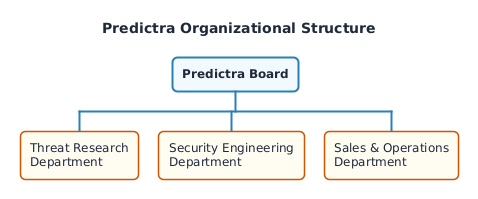
\includegraphics[width=0.9\textwidth]{assets/predictra_org.png}
\caption{Organizational structure of Predictra.}
\label{fig:predictra_org}
\end{figure}

The specific responsibilities of these departments are detailed below:
\begin{itemize}
    \item \textbf{Threat Research Department:} Composed of security analysts and researchers. This department focuses on analyzing cyber campaigns, monitoring extortion websites, and maintaining threat databases. They validate threat indicators and create signatures. Their operations involve examining malware samples, tracking attacker networks, and cataloging actor tactics. Their output is threat intelligence used to feed the ingestion platforms.
    \item \textbf{Security Engineering Department:} Composed of software and database developers. This department is responsible for building ingestion pipelines, data streaming, and the user interface. They focus on database performance, user experience, and cloud deployments. They coordinate with researchers to support new threat indicators.
    \item \textbf{Sales and Operations Department:} Manages client relations, enterprise deployments, marketing campaigns, and commercial threat briefing dissemination, ensuring the platform's features align with commercial market requirements. They gather user feedback from enterprise customers, identify market gaps, and coordinate training and technical support services.
\end{itemize}

\subsection{Inter-Departmental Workflows}
To maintain a high velocity of threat detection and update dissemination, these three departments coordinate via highly structured workflows. When the Threat Research team identifies a new ransomware leak site or an active botnet command-and-control server cluster, they compile the technical signatures and pass them to the Security Engineering team. 

The engineers design new scrapers or update the existing classification databases to support these indicators. Once validated, the engineering team deploys the updates to production environments. Finally, the Sales and Operations team briefs enterprise clients on the newly integrated monitoring capabilities, gathering immediate operational feedback to guide future development iterations.

\section{Project Context and Problem Definition}

Historically, analyzing external threat feeds was a slow, manual process. Threat intelligence teams had to poll separate tabular feeds, manually normalize indicators, and compile static briefings. This tabular approach creates a high **compromise dwell time** -- often exceeding 200 days -- during which adversaries move laterally undetected. Furthermore, Security Operations Center (SOC) analysts suffer from visual fatigue when looking at thousands of static text logs in spreadsheets or simple dashboards. They lack an intuitive, real-time spatial visual interface that provides immediate, global threat situational awareness at a glance.

The \textbf{Predictra Threat Map} was conceived to bridge this critical operational gap, transforming high-velocity, multi-source external cyber threat data into a live, interactive, 3D visual intelligence map and structured analysis dashboard.

\section{State of the Art: Comparative Analysis of CTI Solutions}
To design a robust CTI platform, we conducted a rigorous comparative analysis of existing open-source and commercial threat intelligence solutions, evaluating their data models, stream latencies, spatial visualization support, and hardware footprints.

\subsection{Open-Source Solutions}

\subsubsection{MISP (Malware Information Sharing Platform)}
MISP is a widely used open-source platform for sharing threat information. It supports storing and tagging IP addresses, file hashes, and domains.

From a technical perspective, MISP uses standard database structures. While it is highly capable at storing large lists of historical threats, it is not optimized for real-time streaming. Analysts must request updates periodically, which introduces delays. Furthermore, the user interface consists primarily of text-based tables and lacks real-time 3D visual maps.

Maintaining a MISP instance requires regular management. Security teams must allocate engineering resources to monitor the system and refine database rules. Additionally, because the interface is complex, security teams must spend time training analysts before using it in security operations.

\subsubsection{OpenCTI (Open Cyber Threat Intelligence)}
OpenCTI is a modular platform designed to represent threat intelligence as a graph, linking actors, campaigns, malware, and targeted sectors. It uses specialized databases for indexing and searching, and features connectors to import public and private threat feeds.

However, OpenCTI's architecture is heavy. Running the platform requires managing multiple service layers, which demands high-specification servers and increases operational costs. Furthermore, the interface is optimized for long-term analytical research rather than real-time visual tracking.

From a hosting perspective, the server requirements mean that organizations must allocate significant hardware resources. For smaller teams, this makes the hosting costs high, reducing the financial benefits of using open-source software.

\subsection{Commercial Solutions}

\subsubsection{Recorded Future}
Recorded Future is a major commercial platform that gathers threat indicators from web, forum, and social media channels. It translates these pages into standardized profiles, offering threat scoring and technical indicators, with integrations for major security tools.

Despite its capabilities, Recorded Future is highly expensive, making it inaccessible to smaller organizations. Furthermore, the dashboard is focused on text reports and simple static 2D maps, lacking real-time animations for display screens.

Because it is a closed system, organizations must rely entirely on the vendor's algorithms. Integrating custom data sources not supported by default can be difficult and costly.

\subsubsection{Cyble}
Cyble is a commercial provider focusing on brand protection and monitoring online forums and chat channels for leaked credentials and assets. It provides automated alerts and risk indicators.

Like other commercial options, Cyble requires subscription fees and does not allow custom developer integrations. Its interfaces are designed as static reports, lacking real-time animations, which limits its usefulness for active display environments.

\subsection{Comparative Summary Table}
To clarify the distinctions, a comparative matrix of key platform parameters is detailed in Table~\ref{tab:cti_comparison}.

\begin{table}[H]
\centering
\small
\arrayrulecolor{charcoal!30}
\rowcolors{2}{cyberblue!5}{white}
\begin{tabularx}{\textwidth}{>{\raggedright\arraybackslash}p{2.8cm}XXXX}
\hline
\rowcolor{charcoal}
\thc{Feature / Metric} & \thc{MISP} & \thc{OpenCTI} & \thc{Recorded Future} & \thc{Predictra Threat Map} \\
\hline
Data Model & Attributes / Events & STIX 2.1 Graph~\cite{stix_specification} & Proprietary Graph & Hybrid (SSE + STIX 2.1) \\
Real-Time Streaming & Low (Sync APIs) & Medium (API Poll) & Medium & High (300ms SSE Flush) \\
Visual Spatial Mapping & None & None & Limited 2D Maps & 3D WebGL Globe \& 2D \\
System Resource Footprint & Medium & Very High & N/A (SaaS) & Low (Optimized Node/React) \\
Target Audience & Incident Responders & Intel Analysts & Enterprise SOCs & Modern SOCs \& SMEs \\
Financial Accessibility & Free / Open Source & Free / Open Source & Highly Prohibitive & Open and Accessible \\
\hline
\end{tabularx}
\caption{Academic comparative analysis of global CTI solutions.}
\label{tab:cti_comparison}
\end{table}

\section{Critique of Existing Systems and Proposed Solution}
The evaluation of the state of the art highlights a clear market gap: \textbf{existing CTI platforms are either highly analytical but visually static and resource-heavy (like OpenCTI and MISP), or visually polished but commercially restrictive (like Recorded Future)}. 

To resolve this gap, we proposed the \textbf{Predictra Threat Map}. Our solution is designed as a real-time threat visualizer and analysis workspace:
\begin{itemize}
    \item It uses a modular scraper architecture fetching data from 9+ feeds. This ensures resilience, as the failure of one external feed does not affect others.
    \item It streams events instantly using a coordinated batching queue, keeping browser load low and ensuring smooth data delivery.
    \item It displays an interactive 3D virtual Earth, visualizing threat locations as dynamic curved paths using hardware acceleration.
    \item It integrates a client-side STIX 2.1 file parser, providing analysis features directly in the browser without requiring complex databases.
\end{itemize}

By separating backend data ingestion from frontend visualization and optimizing client-side math, the platform provides high-quality graphics and analysis without requiring expensive server clusters.

\section{Work Methodology and Modeling Standards}
To ensure the rigorous and efficient delivery of this software platform, the project adopted standard industry methodologies for development and system modeling.

\subsection{Agile Scrum Framework}
We implemented the \textbf{Agile Scrum framework} to pilot the development process. This methodology split the project lifecycle into iterative, fully functional increments called \textbf{Sprints}.

\begin{figure}[H]
\centering
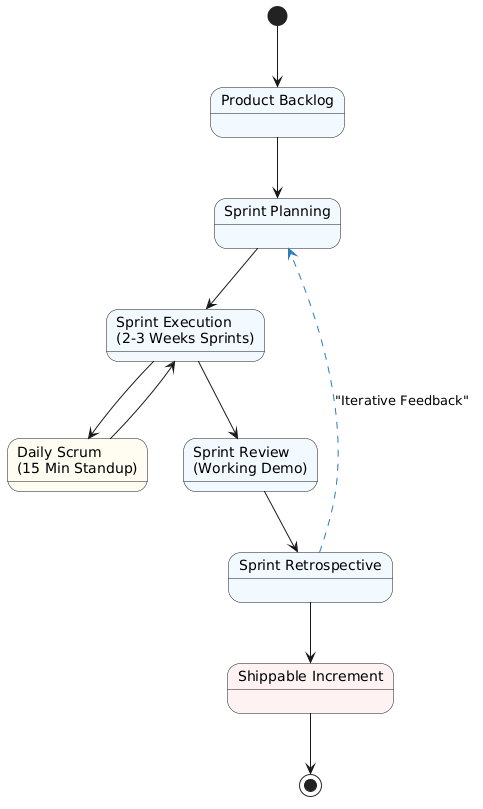
\includegraphics[width=0.8\textwidth]{assets/scrum_lifecycle.png}
\caption{Agile Scrum development lifecycle flowchart.}
\label{fig:scrum_lifecycle}
\end{figure}

The Scrum lifecycle details are structured as follows:
\begin{itemize}
    \item \textbf{Roles:} Brahim Jaballi and Chiheb Amri shared the developer role, with Chiheb coordinating scrum master tasks (sprint planning, daily standups, backlog refinement) and industrial mentors acting as the Product Owner.
    \item \textbf{Sprint Planning (Duration: 2 Hours):} Held at the start of each sprint. The team analyzed the Product Backlog, estimated task complexities using Planning Poker (Fibonacci scale), and committed to a Sprint Backlog. This ritual ensured that the team maintained a clear, realistic set of deliverables for each iteration, avoiding scope creep. Task complexity was evaluated relative to standard reference cards, helping to identify potential design bottlenecks early.
    \item \textbf{Sprint Execution (Duration: 2-3 Weeks):} Active coding, database design, visual design, and integration testing of the committed backlog items. The work was divided using git branch collaborations. The team used continuous integration strategies to ensure that the code on the main branch compiled flawlessly at the end of each day.
    \item \textbf{Daily Scrum (Duration: 15 Minutes):} A daily morning meeting where both team members aligned by answering: What was done yesterday? What will be done today? What are the blockers? This ceremony kept the development highly coordinated and immediately resolved technical bottlenecks, such as library version conflicts or database access permissions.
    \item \textbf{Twice-Weekly Coordination and Review Meetings:} Extended coordination sessions held specifically on Thursdays and Sundays to handle deep code integration, performance profiling, and strategic sprint planning (detailed in Subsection~\ref{subsec:biweekly_meetings}).
    \item \textbf{Sprint Review (Duration: 1.5 Hours):} Conducted at the end of each sprint. The developers demonstrated a working system increment (e.g., the Scraper Pipeline in Sprint 1, the WebGL Globe in Sprint 2) to obtain Product Owner feedback and validate user stories. Any feedback or modification requests were immediately converted into new backlog items.
    \item \textbf{Sprint Retrospective (Duration: 1 Hour):} Held immediately after the review, where the team identified engineering process bottlenecks (e.g. testing bottlenecks, git merge conflicts) and defined continuous improvement action items. This ceremony ensured that team performance improved incrementally with each sprint.
\end{itemize}

\subsection{Twice-Weekly Scrum Coordination and Technical Review Rituals}
\label{subsec:biweekly_meetings}
Because the development of the \textbf{Predictra Threat Map} involved both high-throughput distributed database ingestion systems (scrapers, BSON caches, geocoding) and complex browser-side WebGL canvas renderers, standard 15-minute Daily Scrum meetings were insufficient to resolve dense architectural alignment and integration bottlenecks. To address this, the development team (Brahim Jaballi and Chiheb Amri) instituted an additional twice-weekly extended coordination and technical review cadence, occurring without fail every Thursday and Sunday over the entire six-month project lifecycle (representing over 48 intensive sessions in total).

These bi-weekly sessions acted as the technical anchors of the project. They ensured that both developer branches remained continuously integrated and that any performance bottlenecks (such as garbage collection spikes or memory leaks in the Three.js render loop) were diagnosed and resolved immediately.

\subsubsection{Thursday Technical Alignment Sessions}
The Thursday meetings, typically lasting 3 hours, were positioned at the mid-point of each sprint. Their core purpose was to ensure technical alignment, verify code compilation, and perform peer code reviews. The agenda and operational details are structured below:
\begin{itemize}
    \item \textbf{Code Review and Pull Request Merging:} The developers conducted line-by-line peer reviews of newly written features (e.g., a new scraper module or a UI widget). Branch merges into the local \texttt{develop} environment were executed during this session.
    \item \textbf{API Schema Verification:} External threat intelligence feeds (such as AlienVault OTX or URLhaus) frequently update their JSON fields without notice. Thursdays were used to audit incoming API payloads against our local Mongoose database schemas, resolving any mapping errors or missing geocoding fields.
    \item \textbf{Performance Profiling Sandbox:} Developers ran Chrome DevTools profiling sessions on the rendering thread, checking that the addition of new visual elements (like animated great-circle arcs) did not degrade the rendering framerate below 60fps.
\end{itemize}

\subsubsection{Sunday Strategic Integration and Planning Sessions}
The Sunday meetings, typically lasting 4 hours, were conducted at the end of each weekly cycle. These sessions focused on architectural consolidation, long-term technical planning, and product owner briefings. Their core agenda included:
\begin{itemize}
    \item \textbf{End-of-Week Architectural Refactoring:} Over the course of weekly active coding, developers often introduced minor technical debt. Sundays were dedicated to refactoring complex components, consolidating Zustand store states, cleaning CSS variables, and auditing TypeScript type safety.
    \item \textbf{Academic Documentation Consolidation:} To maintain a high-quality graduation thesis, the team spent the last hour of every Sunday session documenting the technical achievements, designing UML diagrams, and updating the LaTeX report to reflect the current sprint's results.
    \item \textbf{Next-Sprint Planning and Backlog Commitment:} In alignment with upcoming milestones, developers refined the backlog, estimated task sizing using Planning Poker, and committed to the deliverables for the subsequent weekly cycle.
\end{itemize}

To summarize, the operational structure of these twice-weekly coordination sessions is detailed in Table~\ref{tab:biweekly_meetings}.

\begin{table}[H]
\centering
\small
\arrayrulecolor{charcoal!30}
\rowcolors{2}{cyberblue!5}{white}
\begin{tabularx}{\textwidth}{>{\raggedright\arraybackslash}p{2.3cm}XX}
\hline
\rowcolor{charcoal}
\thc{Parameter} & \thc{Thursday Technical Alignment} & \thc{Sunday Strategic Integration} \\
\hline
\textbf{Session Focus} & Technical Integration, Code Auditing, Bug Diagnostics & Architectural Consolidation, Documentation, Sprint Planning \\
\textbf{Typical Duration} & 3.0 Hours & 4.0 Hours \\
\textbf{Key Inputs} & Local Feature Branches, Scraper Output Logs, Performance Metrics & Consolidated \texttt{develop} Branch, Open Backlog, Academic Guide \\
\textbf{Key Activities} & Peer reviews, API schema validation, WebGL frame profiling, branch merging & Code refactoring, Zustand state pruning, LaTeX documentation, backlog sizing \\
\textbf{Primary Output} & Integrated, stable mid-sprint code build & Cleaned production build, updated UML blueprints, next sprint backlog \\
\textbf{Lifespan Coverage} & Every week over 6-month duration (48+ sessions) & Every week over 6-month duration (48+ sessions) \\
\hline
\end{tabularx}
\caption{Operational breakdown of bi-weekly coordination meetings held over 6 months.}
\label{tab:biweekly_meetings}
\end{table}

\subsection{UML Modeling Standards}
To guarantee a solid architectural design, the system requirements, conception, and structure were modeled utilizing the \textbf{Unified Modeling Language (UML)}.
\begin{itemize}
    \item \textbf{Use Case Diagrams:} Captured functional system boundaries and actor-system boundaries. They helped define what services the system must deliver and which human or external actors trigger them, providing a clear map of system responsibilities.
    \item \textbf{Class Diagrams:} Modeled Mongoose database schemas, backend services, and Zustands stores, laying out the structural blueprints of our classes, variables, and methods. These diagrams were crucial in establishing a type-safe structure during TypeScript integrations.
    \item \textbf{Sequence Diagrams:} Traced asynchronous communication timelines between analysts, backend event streams, and front-end render loops, verifying transaction safety and identifying potential race conditions or connection deadlocks.
    \item \textbf{Component Diagrams:} Illustrated modular package boundaries and code dependencies, ensuring a decoupled physical architecture that facilitates scaling.
\end{itemize}

\section{Conclusion}
This chapter established the academic, professional, and methodological foundations of our project. Having analyzed the CTI domain, compared existing market solutions, and set up our Scrum and UML modeling structures, we proceed to Chapter 2 to detail the requirements, project preparation, sprint planning, and the global architecture of the Predictra CTI platform.

\chapter{Project Specification, Planning, and Architecture}

\section{Introduction}
Establishing a robust system requires deep preparation, rigorous specifications, planning, and clean architectural design. This chapter details our functional and non-functional requirements, models the global system needs using a UML Use Case diagram, breaks down the Scrum product backlog, details our development environment, and presents both our infrastructure deployment layout and logical multi-tier application architecture.

\section{Requirements Specification}
To ensure the Predictra Threat Map satisfies academic and operational standards, we captured and defined detailed functional and non-functional requirements.

\subsection{Functional Requirements (RF)}
The platform must support the following nine functional requirements, structured in detail below:

\subsubsection{RF-1: Multi-Feeds Data Ingestion Engine}
\begin{itemize}
    \item \textbf{Description \& Operational Context:} The system must ingest threat events from 9+ external feeds (AlienVault, \allowbreak URLhaus, \allowbreak C2 Tracker, \allowbreak Kaspersky Feodo, \allowbreak Fortinet, \allowbreak Bitdefender, \allowbreak Checkpoint, \allowbreak RansomWatch, \allowbreak and MISP Galaxy), supporting different threat categories (malware, malicious servers, exploits). Collecting data from multiple sources prevents relying on a single vendor, building a more complete threat map. Each external feed utilizes different protocols and data formats. The ingestion layer separates the collection routines, ensuring that a slow query from one feed does not block the collection of others.
    \item \textbf{Use-Case Scenario:} A threat actor registers a new botnet command-and-control server. Within minutes of active staging, the scraper queries the target host, extracts the server details, validates the active listening ports, and pushes the threat indicator into our ingestion pipeline.
    \item \textbf{Inputs:} External threat intelligence feed configurations, API tokens, HTTP endpoints, query rate parameters, connection timeout configurations.
    \item \textbf{Outputs:} Standardized raw threat events JSON packets containing source attributes, raw timestamps, indicator categories, and adversary identification headers.
    \item \textbf{Validation Criteria:} Continuous ingestion from all 9 sources must proceed without data blocking. If an external API goes offline, the scraper must capture the error, log a warning, and schedule a reconnect attempt after a brief delay, preventing server freeze.
\end{itemize}

\subsubsection{RF-2: Geolocation Enrichment Pipeline}
\begin{itemize}
    \item \textbf{Description \& Operational Context:} The backend must automatically find the geographic locations (latitude, longitude, country) of IP addresses using a local geocoding library. Knowing where threats originate helps security teams identify regional attack trends. Because the live stream receives many events per second, resolving locations using online APIs would be too slow and subject to rate limits. Therefore, the geolocation process uses a local database for instant coordinate resolution.
    \item \textbf{Use-Case Scenario:} An incoming exploit log lists the attacker IP \texttt{185.220.101.5}. The geocoder intercepts this address, searches the local IP-to-country database, and resolves the IP to Germany (DE) with coordinates \texttt{51.2993, 9.491}.
    \item \textbf{Inputs:} Raw IP address strings (IPv4 or IPv6 format) extracted from the threat events ingestion queue.
    \item \textbf{Outputs:} ISO two-letter country codes, geocoded Latitude and Longitude decimal coordinates, city name indicators (where available), and Autonomous System Number (ASN) details.
    \item \textbf{Validation Criteria:} Coordinate resolution must execute in low latencies using local caching to avoid external API rate limits. Invalid or private IP blocks (e.g. \texttt{127.0.0.1}) must be mapped to safe default fallback coordinates without raising system exceptions or halting the pipeline execution.
\end{itemize}

\subsubsection{RF-3: Multi-Layer Sector Classification}
\begin{itemize}
    \item \textbf{Description \& Operational Context:} The enrichment engine must dynamically classify threat victims into one of 9 critical business sectors (Healthcare, Finance, Government, Technology, Energy, Education, Telecom, Manufacturing, Retail) using a 5-layer classification engine. This classification allows analysts to filter active threat campaigns targeting their specific vertical. When a cyber threat event occurs, identifying the target industry sector is essential for assessing the systemic risk and cascading impact. For instance, a ransomware attack targeting a financial institution has different regulatory and operational implications compared to a distributed denial-of-service (DDoS) attack targeting a retail website. Since raw feeds rarely contain structured sector tags, the enrichment engine must parse heterogeneous context clues using natural language processing (NLP) keyword matrices, destination port signatures, and historical actor targeting associations to accurately assign a victim sector.
    \item \textbf{Use-Case Scenario:} A RansomWatch scraper indexes an extortion post detailing an attack on "Saint Jude Memorial Hospital." The classifier parses the string, identifies the keyword "Hospital," matches it against the healthcare dictionary, and assigns the target sector to "Healthcare."
    \item \textbf{Inputs:} Attack name, target organization details, destination ports, threat actor profiles, MISP galaxy metadata.
    \item \textbf{Outputs:} Classified target sector name string corresponding to one of the 9 defined critical business sectors.
    \item \textbf{Validation Criteria:} The classification engine must resolve every event within 5 milliseconds. If no sector can be matched via keywords, ports, or metadata, the system must gracefully fall back to the source feed's default sector (such as "Enterprise Technology") to ensure that the event remains categorizable on the threat dashboard.
\end{itemize}

\subsubsection{RF-4: Real-Time Server-Sent Events (SSE) Streaming}
\begin{itemize}
    \item \textbf{Description \& Operational Context:} The server streams geocoded threat events to browsers using a Server-Sent Events (SSE) connection, updating the dashboard instantly without constant polling. Traditional web updates require the browser to request data repeatedly, which is slow and wastes bandwidth. SSE establishes a direct, continuous connection where the server pushes new events to the client. The backend also includes a queue to group and batch incoming threats, ensuring smooth updates.
    \item \textbf{Use-Case Scenario:} A new ransomware victim is indexed. The backend processes the event, enriches it with coordinates, queues it, and immediately flushes it down the open SSE connection, causing the analyst's map to update.
    \item \textbf{Inputs:} Enriched backend threat events from the processing pipeline, active client HTTP connections.
    \item \textbf{Outputs:} HTTP Server-Sent Events (SSE) stream payloads formatted as \texttt{text/}\allowbreak\texttt{event-stream}.
    \item \textbf{Validation Criteria:} Updates must be grouped and flushed at a 300ms interval to protect client browser rendering performance, preventing browser lag from rapid updates. The stream must maintain a keep-alive heartbeat to prevent servers from closing the connection.
\end{itemize}

\subsubsection{RF-5: 3D WebGL Threat Map Visualizer}
\begin{itemize}
    \item \textbf{Description and Context:} The frontend displays an interactive 3D globe showing live attacks as animated curves and pulsating markers, with a toggle to switch to a flat 2D map. A visual threat map is easier to interpret than text logs. The map allows rotation, zooming, and panning. To ensure smooth performance, the visualizer uses hardware acceleration in the browser.
    \item \textbf{Use-Case Scenario:} An analyst mounts the dashboard. A 3D Earth loads in a dark space background, displaying colored lines representing attack vectors between countries.
    \item \textbf{Inputs:} 3D coordinate vectors, attack categories, and time deltas.
    \item \textbf{Outputs:} Interactive 3D visual Earth mesh with glowing arcs, pulsating markers, and country boundary lines.
    \item \textbf{Validation Criteria:} Rendering frame rate must maintain a smooth 60fps under standard attack densities. If the client hardware is low-powered, the system must reduce details to prevent lag.
\end{itemize}

\subsubsection{RF-6: STIX 2.1 Bundle Parser}
\begin{itemize}
    \item \textbf{Description \& Operational Context:} The system must allow analysts to upload standard JSON STIX 2.1 threat intelligence bundles, extract objects (indicators, actors, TTPs), and display them in structured tables. This ensures compliance with global cybersecurity intelligence standards. Standardized threat sharing is essential for collective defense. The Structured Threat Information Expression (STIX) format allows security agencies, CERTs, and private vendors to share threat intelligence without encountering proprietary format blockages. The STIX bundle parser must process complex JSON structures entirely in the browser using client-side JavaScript, ensuring that sensitive enterprise intelligence files are never sent to external servers. The parser must validate the uploaded file structure, extract core STIX domain objects, resolve relationships, and populate the dashboard.
    \item \textbf{Use-Case Scenario:} A government CERT agency releases a STIX bundle concerning a new APT campaign. The analyst uploads the file, extracts the indicators, threat actor profiles, and tools, and reviews them in the structured table.
    \item \textbf{Inputs:} Local STIX 2.1 JSON file uploaded via the dashboard drag-and-drop interface.
    \item \textbf{Outputs:} Isolated maps of STIX objects grouped by threat classes, displayed in interactive, searchable client tables.
    \item \textbf{Validation Criteria:} The parser must validate the JSON schema, ensure the presence of required fields (such as \texttt{spec\_version: "2.1"} and \texttt{type: "bundle"}), and seamlessly support large files (up to 300KB) entirely client-side without locking the browser's main execution thread.
\end{itemize}

\subsubsection{RF-7: MITRE ATT\&CK Kill Chain Mapping}
\begin{itemize}
    \item \textbf{Description \& Operational Context:} The STIX dashboard must map extracted adversary techniques directly into the 12 phases of the MITRE ATT\&CK Cyber Kill Chain, illustrating threat distributions per phase. This categorization assists teams in planning security remediation. The MITRE ATT\&CK matrix is the industry-standard taxonomy for cataloging adversary tactics, techniques, and procedures (TTPs). By mapping ingested STIX attack pattern objects directly to this matrix, the platform provides security teams with immediate visibility into the adversary's operational phase. For example, if a parsed bundle contains an overwhelming number of techniques concentrated in the "Initial Access" phase, defenders know they must focus on perimeter controls. If the techniques are clustered in "Privilege Escalation," internal endpoint security must be audited.
    \item \textbf{Scenario:} The parsed STIX bundle contains techniques like "Spearphishing Link" and "DLL Side-Loading". The matrix groups them under "Initial Access" and "Defense Evasion" respectively, displaying a visual count indicator in the UI grid.
    \item \textbf{Inputs:} Parsed STIX attack pattern objects containing MITRE ATT\&CK \texttt{kill\_}\allowbreak\texttt{chain\_}\allowbreak\texttt{phases} identifiers.
    \item \textbf{Outputs:} Structured 12-phase MITRE ATT\&CK visual matrix showing technique distributions and descriptive popups.
    \item \textbf{Validation Criteria:} Distribution counts per phase must update automatically upon parsing, highlighting the most heavily populated stages to focus mitigation efforts. Malformed or custom phase names must be safely grouped under an "Other / Custom" column to prevent grid rendering failures.
\end{itemize}

\subsubsection{RF-8: Searchable Historical Database Browser}
\begin{itemize}
    \item \textbf{Description \& Operational Context:} The platform must provide a searchable historical log viewer of persisted threat records, filtering by country, target sector, IP address, and free-text regex queries, with paging to protect server performance. Real-time visual monitoring must be backed by a strong historical record system. When a security incident is detected, investigators must query historical logs to perform forensic audits, searching if similar threat vectors have targeted their infrastructure in the past. To ensure high speed, the database queries must leverage indexes on frequently searched fields. The interface must provide paginated views to protect server and client memory from massive document arrays.
    \item \textbf{Use-Case Scenario:} An investigator searches for all "Healthcare" threats originating from "Russia" (RU) during the last week, filtering the results instantly in a searchable table.
    \item \textbf{Inputs:} Search strings, country selection, target sector, pagination index parameters.
    \item \textbf{Outputs:} Paginated BSON threat documents array matching the query filters.
    \item \textbf{Validation Criteria:} Query page size must be bounded (default 50 logs per page) to prevent server memory bloat, with database queries executing in under 50ms using indexing.
\end{itemize}

\subsubsection{RF-9: Target My IP Helper \& Excel Export}
\begin{itemize}
    \item \textbf{Description \& Operational Context:} The history page must integrate a quick-helper to geolocate and query threats targeting the investigator's public IP, alongside a feature to export threat logs into formatted Microsoft Excel files. Analysts often need to run quick sanity checks on their local networks or export forensic evidence for presentation to stakeholders. The "Target My IP" helper queries an external public IP API, geolocates the client, and automatically searches the threat history database to identify if their specific public network IP or neighboring subnet blocks have been logged as active targets by any scraper. The Excel export feature converts current query results into standard XML Spreadsheet formats entirely client-side.
    \item \textbf{Use-Case Scenario:} An analyst wants to see if their current network has been targeted. They click "Target My IP," geolocate themselves, filter the logs, and export the threat list to Excel for a security briefing.
    \item \textbf{Inputs:} Clicked HUD buttons, public IP query results.
    \item \textbf{Outputs:} Geolocated public client IP and formatted Excel spreadsheet downloads.
    \item \textbf{Validation Criteria:} Export must support up to 5,000 logs in a single continuous stream utilizing fast client-side worksheet packages, preventing browser memory exhaustion.
\end{itemize}

\subsection{Non-Functional Requirements (RNF)}
To satisfy system reliability, performance, and aesthetic standards, five non-functional requirements were established:

\begin{subsubsection}{RNF-1: High Frame-Rate and UI Fluidity}
The 3D globe should run smoothly at 60 frames per second (FPS). The frontend must implement adaptive checks, dynamically reducing visual details if the frame rate drops, ensuring that map controls remain responsive.
\end{subsubsection}

\begin{subsubsection}{RNF-2: Minimal Memory Footprint}
The client dashboard must manage memory efficiently. The system uses a circular buffer with a maximum capacity of 10,000 events to store data. This buffer overrides old events in-place, keeping memory usage constant and avoiding performance stutters.
\end{subsubsection}

\begin{subsubsection}{RNF-3: Self-Cleaning Storage \& Time-To-Live (TTL)}
The database growth must be bounded. Old threat records must automatically expire and prune from the database after a 30-day Time-To-Live (TTL) interval, avoiding billing overages on free cloud database tiers.
\end{subsubsection}

\begin{subsubsection}{RNF-4: Database Storage Quota Guard}
The backend monitors the database collection size. If database storage exceeds 500 MB, the server automatically stops database writes and switches to in-memory streaming to prevent database errors.
\end{subsubsection}

\begin{subsubsection}{RNF-5: Glassmorphism UI Theme}
The interface implements a modern dark theme design, utilizing semi-transparent panel styles and colors based on threat severity, which reduces eye strain and provides a clean visual workspace.
\end{subsubsection}

\section{System Needs Modeling}
To define the system boundary, we identified the primary actors and modeled their interactions with the global platform using a UML Use Case diagram.

\subsection{Identification of Actors}
We identified two main actors interacting with our system:
\begin{itemize}
    \item \textbf{External Threat Feeds (System Actor):} Ingests raw cyber threat logs via HTTP REST APIs, SSE feeds, or WebSockets. It acts as the primary data supplier.
    \item \textbf{Security Analyst (Human Actor):} Interacts with the frontend dashboard to monitor geolocated threat vectors, explore history, export data, and upload/explore STIX 2.1 threat intelligence bundles.
\end{itemize}

\subsection{Global Use Case Diagram}
The global interactions are illustrated in the UML Use Case diagram in Figure~\ref{fig:global_usecase}.

\begin{figure}[H]
\centering
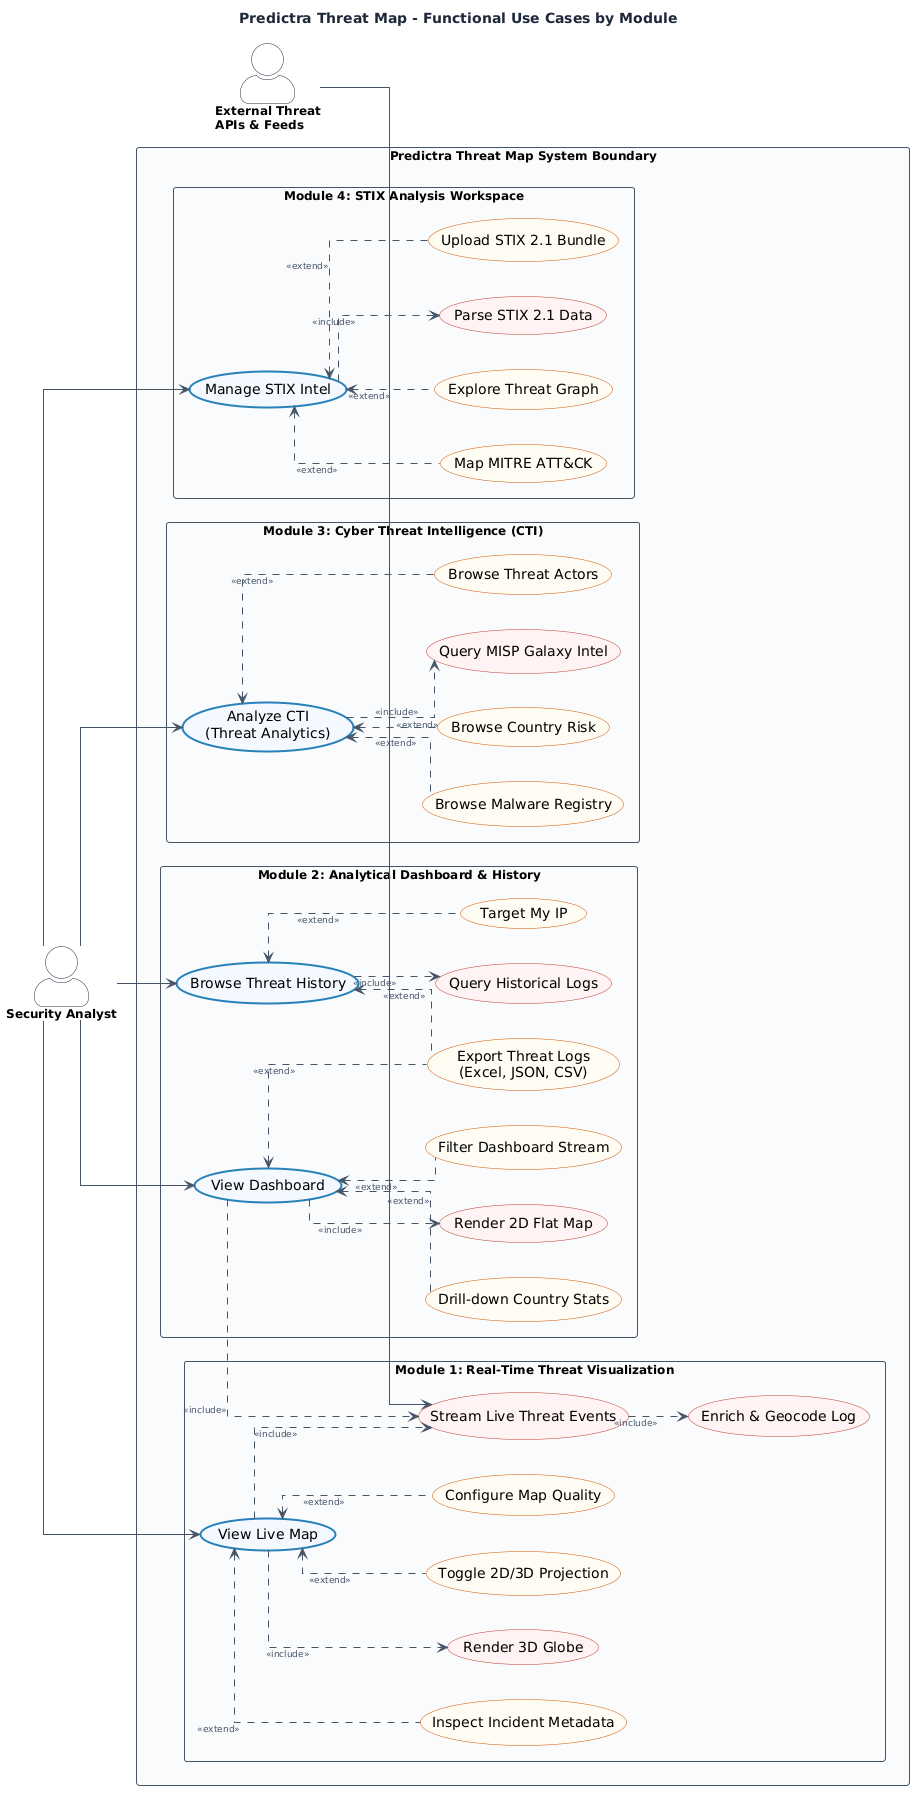
\includegraphics[width=\textwidth,height=0.85\textheight,keepaspectratio]{assets/global_usecase.png}
\caption{UML Global Use Case diagram for the Predictra CTI platform.}
\label{fig:global_usecase}
\end{figure}

The specific functional workflows of these use cases are summarized in Table~\ref{tab:global_uc_desc}.

\begin{table}[H]
\centering
\small
\arrayrulecolor{charcoal!30}
\rowcolors{2}{cyberblue!5}{white}
\begin{tabularx}{\textwidth}{>{\raggedright\arraybackslash}p{3.2cm}>{\raggedright\arraybackslash}p{3.5cm}X}
\hline
\rowcolor{charcoal}
\thc{Base Use Case} & \thc{Included / Extending} & \thc{Main Workflow \& Interaction Details} \\
\hline
View Live Map &
\textbf{Includes:} Stream Live Events, Render 3D Globe \newline
\textbf{Extends:} Toggle 2D/3D Projection, Configure Map, Inspect Metadata &
Security Analyst mounts the map view. The frontend initiates the WebGL globe render loop and hooks into the Server-Sent Events (SSE) client stream. Optional controls allow altering atmospheric/trail quality, flattening coordinates to 2D Mercator, and hovering over bezier arcs to see raw metadata. \\
\midrule
View Dashboard &
\textbf{Includes:} Stream Live Events, Render 2D Flat Map \newline
\textbf{Extends:} Filter Dashboard, Drill-down Country, Export Logs &
Security Analyst opens the flat command center view. System displays grid panels containing real-time metrics, sparklines, and maps. Analyst can query events using regex, click countries to see drill-down reports, or export the active buffer to JSON, CSV, or formatted Excel sheets. \\
\midrule
Browse Threat History &
\textbf{Includes:} Query Historical Logs \newline
\textbf{Extends:} Target My IP, Export Logs &
Security Analyst searches the persistent database. System queries MongoDB Atlas collections. Helper features allow automated public IP geolocation checks (Target My IP) to query matching subnet logs and client-side formatting for Excel spreadsheet exports. \\
\midrule
Analyze CTI \newline (Threat Analytics) &
\textbf{Includes:} Query MISP Galaxy \newline
\textbf{Extends:} Browse Actors, Browse Malware, Browse Country Risk &
Security Analyst accesses the threat intelligence portal. The system retrieves stored MISP Galaxy templates. The analyst filters APT groups by country attribution or target sector, audits ransomware encryption details, and views geographical vulnerability heatmaps. \\
\midrule
Manage STIX Intel &
\textbf{Includes:} Parse STIX 2.1 \newline
\textbf{Extends:} Upload STIX, Map MITRE &
Security Analyst mounts the STIX 2.1 analysis environment. The analyst uploads a JSON bundle, parsed client-side. The frontend maps adversary patterns into the 12 phases of the MITRE ATT\&CK Cyber Kill Chain. \\
\hline
\end{tabularx}
\caption{Detailed descriptions of the global primary use cases and their relationships.}
\label{tab:global_uc_desc}
\end{table}

\clearpage

\section{Project Management with Scrum}
As described in Chapter 1, we implemented the Agile Scrum methodology to pilot the design and realization.

\subsection{Product Backlog}
The features requested by the Product Owner were broken down into four distinct sprint backlogs:
\begin{itemize}
    \item \textbf{Sprint 1 (Ingestion Backend):} Setup Express backend server, database schemas, MongoDB Atlas connections, 9 parallel REST/stream scrapers, and the 5-layer sector classification pipeline. Focus on high-throughput database inserts and robust API connection pooling.
    \item \textbf{Sprint 2 (Visualizer Frontend 3D Earth):} Develop the Express SSE feed endpoint with 300ms queue, establish the Zustand store on the React frontend, and build the 3D procedural WebGL Earth Canvas with bloom rendering, bezier fly-arcs, and pulsating markers. Target a smooth 60fps orbital rotation.
    \item \textbf{Sprint 3 (STIX Analysis Workspace):} Create the frontend STIX 2.1 JSON parser and implement the MITRE ATT\&CK Kill Chain mapping. Focus on client-side parsing performance and kill chain validation.
    \item \textbf{Sprint 4 (Analytics, History \& Performance Polish):} Setup the historical log browser, code "Target My IP" geolocator, integrate MISP threat actor datasets, write Excel export streams, and implement performance safeguards (RingBuffer, Zustand throttler, and adaptive FPS sampling drops).
\end{itemize}

\subsection{Previsional Gantt Chart}
Our chronological sprint schedule is modeled in Figure~\ref{fig:gantt_chart} using a timeline chart.

\begin{figure}[H]
\centering
\begin{tikzpicture}[x=0.95cm, y=0.85cm]

  % ─── constants ────────────────────────────────────────────────────
  \def\nrows{4}   % number of sprint rows
  \def\ncols{12}  % total weeks
  \def\lw{2.6}    % left-label column width (in x-units, shifted)

  % ─── alternating row backgrounds ──────────────────────────────────
  \fill[gray!8]  (0, 0) rectangle (\ncols, 1);
  \fill[white]   (0, 1) rectangle (\ncols, 2);
  \fill[gray!8]  (0, 2) rectangle (\ncols, 3);
  \fill[white]   (0, 3) rectangle (\ncols, 4);

  % ─── outer border ─────────────────────────────────────────────────
  \draw[charcoal!40, line width=0.7pt] (0,0) rectangle (\ncols, 4);

  % ─── vertical week separator lines ────────────────────────────────
  \foreach \w in {1,2,...,11} {
    \draw[gray!30, line width=0.35pt] (\w, 0) -- (\w, 4);
  }

  % ─── horizontal row separator lines ───────────────────────────────
  \foreach \r in {1,2,3} {
    \draw[gray!30, line width=0.35pt] (0, \r) -- (\ncols, \r);
  }

  % ─── header row ───────────────────────────────────────────────────
  \fill[charcoal!12] (0,4) rectangle (\ncols, 4.55);
  \draw[charcoal!40, line width=0.7pt] (0,4) rectangle (\ncols, 4.55);
  \foreach \w in {1,...,12} {
    \node[font=\footnotesize\bfseries, text=charcoal]
      at (\w-0.5, 4.275) {W\w};
  }

  % ─── row label column header ───────────────────────────────────────
  % (drawn to the left of x=0)
  \fill[charcoal!12] (-\lw, 0) rectangle (0, 4.55);
  \draw[charcoal!40, line width=0.7pt] (-\lw, 0) rectangle (0, 4.55);
  \draw[charcoal!40, line width=0.5pt] (-\lw, 4) -- (0, 4);
  \node[font=\footnotesize\bfseries, text=charcoal] at (-\lw/2, 4.275) {Sprint};

  % row dividers in label column
  \foreach \r in {1,2,3} {
    \draw[gray!30, line width=0.35pt] (-\lw, \r) -- (0, \r);
  }

  % ─── sprint row labels ─────────────────────────────────────────────
  \node[font=\small\bfseries, text=charcoal, align=center]
    at (-\lw/2, 3.5) {\#1};
  \node[font=\small\bfseries, text=charcoal, align=center]
    at (-\lw/2, 2.5) {\#2};
  \node[font=\small\bfseries, text=charcoal, align=center]
    at (-\lw/2, 1.5) {\#3};
  \node[font=\small\bfseries, text=charcoal, align=center]
    at (-\lw/2, 0.5) {\#4};

  % ─── Sprint bars ──────────────────────────────────────────────────
  % Sprint 1: Weeks 1-3, Row 4 (y=3..4)
  \fill[cyberblue!30, rounded corners=3pt]
    (0.08, 3.14) rectangle (2.92, 3.86);
  \draw[cyberblue!70, line width=0.8pt, rounded corners=3pt]
    (0.08, 3.14) rectangle (2.92, 3.86);
  \node[font=\scriptsize\bfseries, text=charcoal, align=center,
         text width=2.6cm]
    at (1.5, 3.5) {Harvester\\Backend};

  % Sprint 2: Weeks 4-6, Row 3 (y=2..3)
  \fill[cyberblue!48, rounded corners=3pt]
    (3.08, 2.14) rectangle (5.92, 2.86);
  \draw[cyberblue!80, line width=0.8pt, rounded corners=3pt]
    (3.08, 2.14) rectangle (5.92, 2.86);
  \node[font=\scriptsize\bfseries, text=charcoal, align=center,
         text width=2.6cm]
    at (4.5, 2.5) {3D Visualizer};

  % Sprint 3: Weeks 7-9, Row 2 (y=1..2)
  \fill[cyberblue!66, rounded corners=3pt]
    (6.08, 1.14) rectangle (8.92, 1.86);
  \draw[cyberblue!90, line width=0.8pt, rounded corners=3pt]
    (6.08, 1.14) rectangle (8.92, 1.86);
  \node[font=\scriptsize\bfseries, text=charcoal, align=center,
         text width=2.6cm]
    at (7.5, 1.5) {STIX Parser};

  % Sprint 4: Weeks 10-12, Row 1 (y=0..1)
  \fill[cyberblue!88, rounded corners=3pt]
    (9.08, 0.14) rectangle (11.92, 0.86);
  \draw[cyberblue, line width=0.8pt, rounded corners=3pt]
    (9.08, 0.14) rectangle (11.92, 0.86);
  \node[font=\scriptsize\bfseries, text=white, align=center,
         text width=2.6cm]
    at (10.5, 0.5) {Analytics\\\& Polish};

\end{tikzpicture}
\caption{Previsional Gantt Chart of development sprints.}
\label{fig:gantt_chart}
\end{figure}

\section{Work Environment}
To support development and testing, we established a standardized hardware and software environment.

\subsection{Hardware Environment}
\begin{itemize}
    \item \textbf{Development Workstation:} Intel Core i7 12th Generation Processor, 16 GB DDR4 RAM, 512 GB NVMe SSD, Nvidia GeForce RTX 3060 Laptop GPU (essential for rendering and debugging high-velocity WebGL atmospheric fragment shaders and real-time bloom post-processing filters without interface lagging).
    \item \textbf{Staging Test Server:} Dual-core Virtual Private Server representing cloud staging infrastructure.
\end{itemize}

\subsection{Software Environment and Development Tools}
\begin{itemize}
    \item \textbf{Operating System:} Windows 11 Home for developer environments, Linux Ubuntu Server 22.04 LTS for cloud API staging processes.
    \item \textbf{IDE:} Visual Studio Code (VS Code) with TypeScript ESLint, Git, and LaTeX Workshop extensions.
    \item \textbf{Database Inspection:} MongoDB Compass for inspecting Mongoose models and TTL indexes, and Robo 3T.
    \item \textbf{API Testing:} Postman for constructing mock threat streams and auditing Server-Sent Events headers.
\end{itemize}

\subsection{Stack and Frameworks Comparative Analysis}
The selection of our development stack was not arbitrary; it was the result of a rigorous architectural evaluation designed to balance the competing demands of high-throughput backend data harvesting and ultra-smooth, lightweight frontend WebGL rendering. Every framework and language was scrutinized against standard industry alternatives to ensure optimal resource efficiency.

\subsubsection{Core Languages: Type Safety vs. Volatile Scripting}
For backend development, we used JavaScript to handle the incoming data formats which can vary in structure. On the client side, we implemented TypeScript to provide structure and type-checking, preventing runtime errors that could crash the interface.

\subsubsection{Backend Environment: Node.js/Express vs. Java Spring Boot / Go}
We selected Node.js with Express instead of heavy enterprise environments like Java Spring Boot or Go:
\begin{itemize}
    \item \textbf{Comparison with Spring Boot:} Spring Boot allocates substantial server resources for each connection. In our case, where we maintain continuous connections for streaming threat data, this would consume significant memory.
    \item \textbf{Comparison with Go:} While Go is fast, Node.js provides a large ecosystem of libraries for database mapping, geocoding, and REST requests, allowing faster development.
    \item \textbf{Node.js Advantages:} Node.js is designed to handle thousands of concurrent client connections efficiently under a low memory footprint, making it ideal for streaming threat feeds in real-time.
\end{itemize}

\subsubsection{Frontend Engine: React 19 \& Vite 7 vs. Webpack / Next.js}
For the client-side interface, we used React with Vite instead of Webpack or Next.js:
\begin{itemize}
    \item \textbf{Next.js:} Next.js is optimized for page pre-rendering and SEO, which is not needed for a real-time visual application where all data updates dynamically in the browser.
    \item \textbf{Vite vs. Webpack:} Webpack compiles all assets before starting, which is slow. Vite compiles code on-demand, providing faster startup times and quicker updates during development.
\end{itemize}

\subsubsection{3D Graphics: Three.js and React Three Fiber (R3F)}
To display the 3D globe with many overlapping lines and markers, we used Three.js via React Three Fiber (R3F). R3F allows building 3D meshes using React components, handling resizing and camera controls automatically while keeping the performance high.

\subsubsection{State Management: Zustand 5 vs. Redux Toolkit}
To manage real-time threat data in the browser, we chose Zustand over Redux Toolkit. Redux triggers full-page render updates, which slows down performance when receiving multiple events per second. Zustand allows direct updates to the 3D canvas components, keeping the interface smooth.

\subsubsection{Data Persistence: MongoDB Atlas BSON vs. SQL Relational Databases}
For database storage, we utilized MongoDB instead of relational databases like PostgreSQL or MySQL. Relational databases require rigid table structures, which is difficult because threat data from different scrapers contains different fields. MongoDB allows storing flexible document structures, making it easier to integrate new feeds.

\subsubsection{Technology Stack Comparative Summary Matrix}
To formalize the architectural rationale behind our technology choices, a detailed comparison matrix evaluating our selected stack against traditional enterprise alternatives is presented in Table~\ref{tab:tech_stack_comparison}.

\begin{table}[H]
\centering
\small
\arrayrulecolor{charcoal!30}
\rowcolors{2}{cyberblue!5}{white}
\begin{tabularx}{\textwidth}{>{\raggedright\arraybackslash}p{2.2cm}>{\raggedright\arraybackslash}p{2.5cm}>{\raggedright\arraybackslash}p{2.5cm}X}
\hline
\rowcolor{charcoal}
\thc{Layer / Component} & \thc{Selected Technology} & \thc{Traditional Alternative} & \thc{Architectural Rationale for Selection} \\
\hline
\textbf{Runtime Engine} & Node.js LTS (v20) \& Express 5 & Java Spring Boot & Asynchronous non-blocking event-driven loop vs heavy Thread-per-Request. Scalable for open SSE streams under low memory. \\
\textbf{State Management} & Zustand 5 & Redux Toolkit & Slice-based reactive updates outside React DOM rendering vs full-tree dispatches. Essential for preserving 60fps WebGL rendering. \\
\textbf{Graphics Engine} & Three.js \& React Three Fiber & Vanilla HTML5 Canvas & Declarative component composition, GPU acceleration, SLERP math, and custom GLSL vertex/fragment shaders. \\
\textbf{Client Build Tool} & React 19 \& Vite 7 & Angular \& Webpack & Native ESM during dev, instant startup, fast HMR updates vs slow dependency pre-compilation graphs. \\
\textbf{Data Persistence} & MongoDB Atlas (BSON) & PostgreSQL / MySQL & Dynamic schemaless BSON documents for heterogeneous CTI logs vs rigid relational tables requiring heavy migrations. \\
\hline
\end{tabularx}
\caption{Comprehensive architectural comparison of selected vs alternative technologies.}
\label{tab:tech_stack_comparison}
\end{table}

\section{Architectural Design}
To guarantee maximum horizontal scalability and system responsiveness under high threat ingestions, we adopted a clean, modular multi-tier architecture.

\subsection{Deployment Architecture}
The system deployment model is structured into three cloud layers:
\begin{enumerate}
    \item \textbf{Frontend Layer (Vercel CDN):} The single-page application is hosted on Vercel's global Content Delivery Network. The configuration file `vercel.json` intercepts client requests and handles API proxy rewrites directly, as summarized in Table~\ref{tab:vercel_proxy} (with the full production configuration file detailed in Appendix D.1).
    \item \textbf{Backend Layer (Virtual Cloud VM):} The Node.js Express server runs as a continuous service managed by PM2 on a secure virtual instance. PM2 clusters the Node process across multiple virtual CPU cores, routing client requests and handling automated crash recoveries.
    \item \textbf{Database Layer (MongoDB Atlas Cluster):} persistence is offloaded to a replicated MongoDB Atlas cloud cluster, handling scalable BSON document writes.
\end{enumerate}

\begin{table}[H]
\centering
\small
\arrayrulecolor{charcoal!30}
\rowcolors{2}{cyberblue!5}{white}
\begin{tabular}{ll}
\hline
\rowcolor{charcoal}
\thc{Source Match Rule} & \thc{Target VM Service Endpoint} \\
\hline
\texttt{/api/:path*} & \texttt{http://api:3001/api/:path*} \\
\hline
\end{tabular}
\caption{Frontend Reverse-Proxy Routing Configuration.}
\label{tab:vercel_proxy}
\end{table}

\subsection{System Package Component Architecture}
To ensure clean separation of concerns, our physical system is organized into decoupled modules, as illustrated in the UML Component diagram in Figure~\ref{fig:component_diagram}.

\begin{figure}[H]
\centering
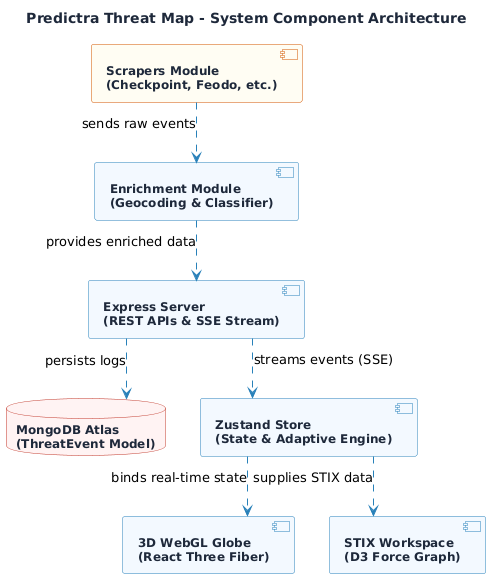
\includegraphics[width=0.95\textwidth]{assets/component_diagram.png}
\caption{UML Component diagram of the Predictra CTI system.}
\label{fig:component_diagram}
\end{figure}

\subsection{Application Logical Architecture}
The Predictra Threat Map's internal logic is partitioned into 4 distinct tiers, as illustrated in the logical architecture diagram in Figure~\ref{fig:logical_architecture}.

\begin{figure}[H]
\centering
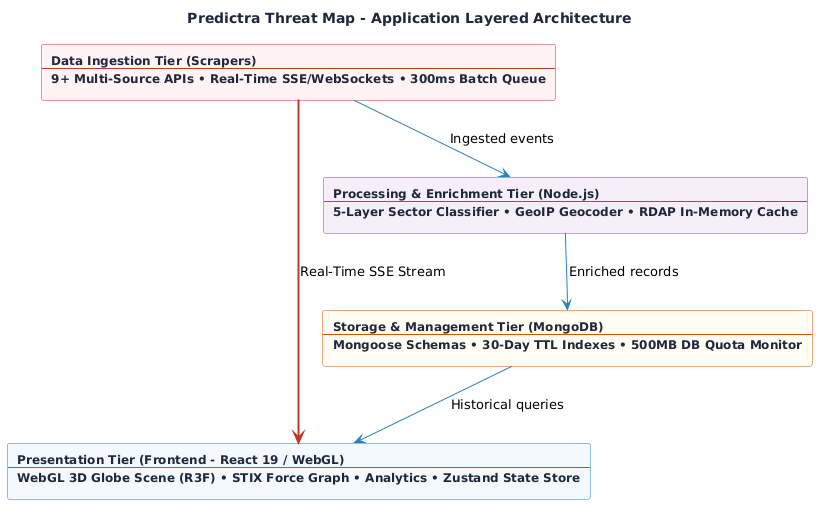
\includegraphics[width=0.95\textwidth]{assets/multi_tier_architecture.png}
\caption{Predictra platform multi-tier layered application architecture.}
\label{fig:logical_architecture}
\end{figure}

This multi-tier structure enforces strict data-flow boundaries:
\begin{itemize}
    \item \textbf{Data Isolation:} Ingestion processes are decoupled from main database queries. Scrapers fetch raw feeds independently, queuing items to prevent memory locks.
    \item \textbf{Decoupled Presentation:} The WebGL client consumes the live stream directly via the SSE pipeline. This bypasses long-term storage routes, ensuring that high database writes do not interfere with 3D canvas responsiveness.
\end{itemize}

\subsection{Global Class Diagram}
To model the static structure of the Predictra CTI system, we designed a Global Class Diagram that illustrates the key logical modules, their core attributes, operational methods, and structural relationships. The diagram is illustrated in Figure~\ref{fig:global_class_diagram}.

\begin{figure}[H]
\centering
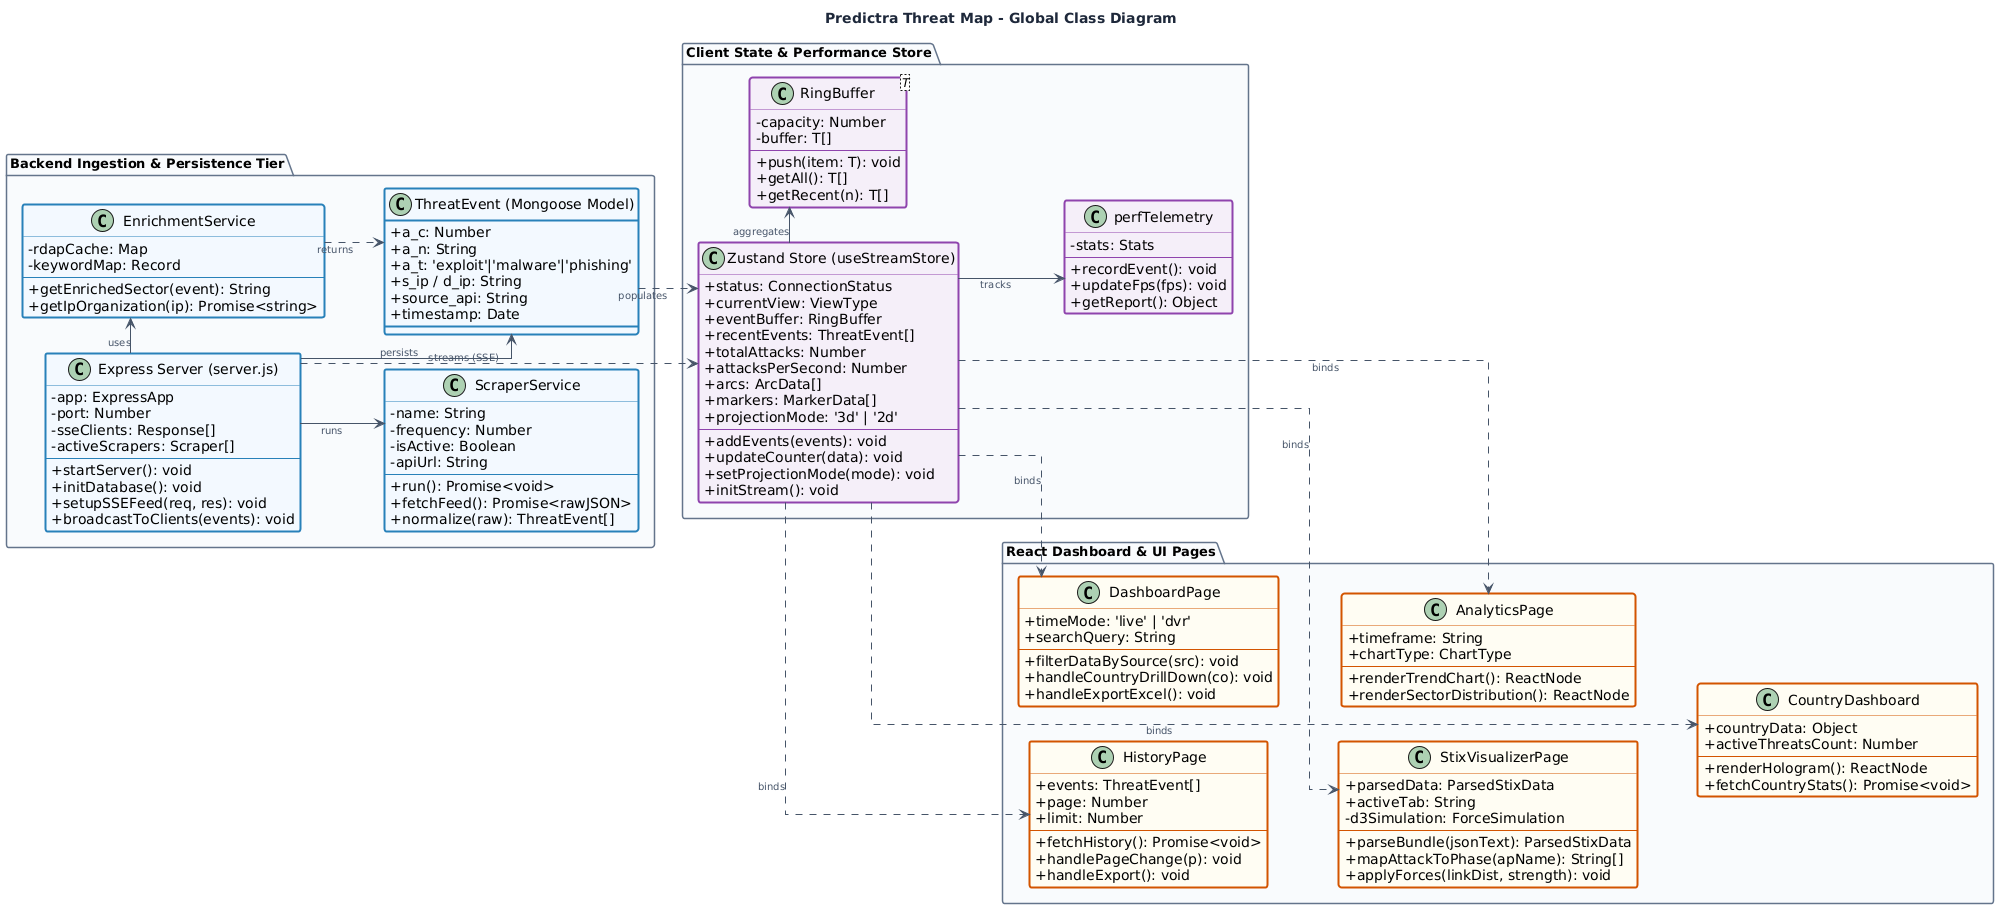
\includegraphics[width=0.95\textwidth]{assets/global_class_diagram.png}
\caption{UML Global Class diagram of the Predictra CTI system.}
\label{fig:global_class_diagram}
\end{figure}

The structural design modeled in Figure~\ref{fig:global_class_diagram} highlights several key object-oriented associations, compositions, and structural dependencies across the three main tiers of our application:
\begin{itemize}
    \item \textbf{Backend Ingestion \& Persistence Tier:} The central \texttt{Express Server} instantiates and schedules multiple concurrent \texttt{ScraperService} instances (e.g. \texttt{Urlhaus}, \texttt{AlienVault}, \texttt{MispGalaxy}, \texttt{Ransomwatch}). As threat telemetry is gathered, it is processed via the \texttt{EnrichmentService} which resolves network organizations and classifies critical infrastructure sectors. The server then persists the resulting dataset using the Mongoose \texttt{ThreatEvent} data model, maintaining standard index rules.
    \item \texttt{Zustand Store} and performance utilities: The client-side \texttt{useStreamStore} acts as a real-time reactive state manager. To handle incoming threat stream data without memory leaks or high garbage collection cycles, the store encapsulates a circular \texttt{RingBuffer} class structure and tracks performance through the custom instrumented \texttt{perfTelemetry} class.
    \item \textbf{React Views Tier:} React pages and tab elements represent the core view controllers. The \texttt{DashboardPage}, \texttt{HistoryPage}, \texttt{AnalyticsPage}, \texttt{StixDashboard}, and \texttt{CountryDashboard} subscribe to the Zustand store state slices and bind to specific endpoints (like \texttt{/api/history} and \texttt{/api/stats}) to drive layout changes and charts.
\end{itemize}

\section{Conclusion}
This chapter established the complete blueprints of our CTI platform. Having documented the functional/non-functional specifications, structured the Scrum timelines, cataloged our dev environment, and detailed our layered deployment and application logical architectures, we proceed to Chapter 3 to document the deep implementation details and UML structures of our first Release.

\chapter{First Release - Core Ingestion and 3D Visualization}

\section{Introduction}
This chapter documents the design, modeling, and realization of the first functional release of the platform, aligning with the \textbf{Release 1} specifications. This release covers \textbf{Sprint 1 (Core Data Ingestion and Scraper Pipeline)} and \textbf{Sprint 2 (Real-Time SSE Streaming and 3D Globe Visualization)}. For each sprint, we present its backlog objectives, UML modeling diagrams (Use Case, Class, and Sequence), database schemas, component structures, code walks, and interface screenshots.

---

\section{Sprint 1: Data Ingestion and Enrichment Pipeline}

\subsection{Sprint Backlog and Objectives}
The core objective of Sprint 1 was to establish the ingestion backend. This included configuring the Express server, setting up Mongoose models, coding the 9 modular scrapers, and implementing the 5-layer sector classification and geolocation enrichment pipeline. 

The primary engineering challenges in this sprint involved managing parallel connections to heterogeneous APIs and transforming varying, unstructured data formats into a unified, compact database schema, ensuring database writes remained performant under high threat volumes.

\subsection{Sprint Analysis: Use Case Modeling}
The ingestion use cases are captured in Figure~\ref{fig:s1_usecase}, illustrating how the External API Feed actor triggers the harvest loop.

\begin{figure}[htbp]
\centering
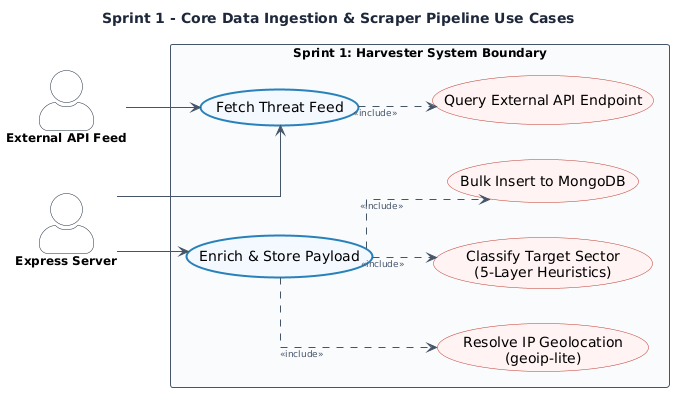
\includegraphics[width=0.95\textwidth]{assets/s1_usecase.png}
\caption{Sprint 1: Use Case diagram for threat data harvesting.}
\label{fig:s1_usecase}
\end{figure}

The functional behaviors of these use cases are structured in Table~\ref{tab:s1_uc_desc}.

\begin{table}[htbp]
\centering
\small
\begin{tabular}{>{\raggedright\arraybackslash}p{3.8cm}>{\raggedright\arraybackslash}p{4.7cm}>{\raggedright\arraybackslash}p{4.7cm}}
\toprule
\textbf{Use Case} & \textbf{Actor/Trigger} & \textbf{Main Workflow} \\
\midrule
Fetch Threat Feed & Express Server (Scheduler / Poll) & The server initiates a scheduler, calling a modular scraper file to query the external REST endpoint or establish a streaming connection, retrieving threat JSON packets. \\
Enrich \& Store Payload & Express Server (Callback / Data In) & Upon retrieval, the payload is resolved through `enrichment.js` for IP geolocation and target sector classification, and queued for bulk MongoDB write. \\
\bottomrule
\end{tabular}
\caption{Sprint 1: Use Case descriptions.}
\label{tab:s1_uc_desc}
\end{table}

\subsection{Sprint Conception: Classes, Sequences, and Schemas}

\subsubsection{UML Class Diagram}
The structural interfaces created in Sprint 1 are illustrated in Figure~\ref{fig:s1_class}.

\begin{figure}[htbp]
\centering
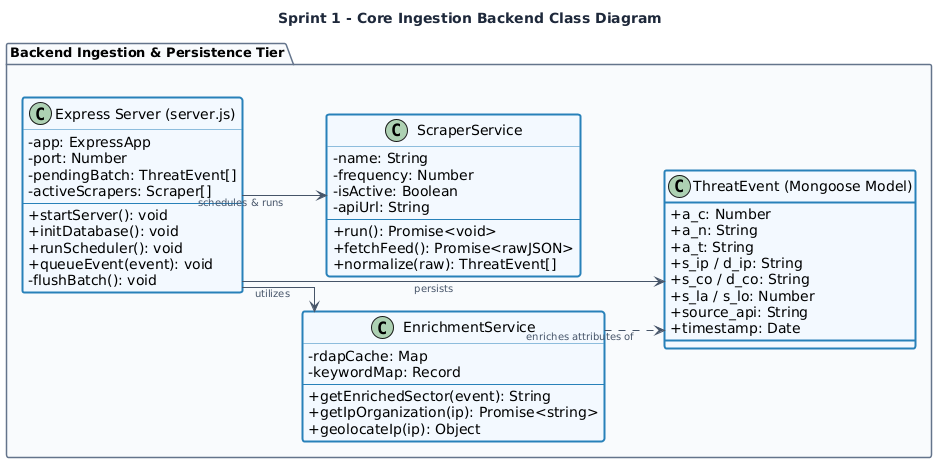
\includegraphics[width=0.95\textwidth]{assets/s1_class.png}
\caption{Sprint 1: Conception Class diagram.}
\label{fig:s1_class}
\end{figure}

\subsubsection{MongoDB Schema Dictionary}
To accommodate high-velocity database writes (up to hundreds of logs per second), the MongoDB schema in `models/ThreatEvent.js` uses \textbf{compact field names} to minimize BSON document sizes. This layout reduces document sizes from 200 bytes to 80 bytes, conserving cloud database storage. Furthermore, a compound index was established on `s\_ip` and `timestamp` to accelerate fast queries on the history explorer page. The database schema dictionary mapping is defined in Table~\ref{tab:db_dictionary}.

\begin{table}[htbp]
\centering
\small
\begin{tabular}{>{\raggedright\arraybackslash}p{3.2cm}>{\raggedright\arraybackslash}p{2.0cm}>{\raggedright\arraybackslash}p{1.4cm}>{\raggedright\arraybackslash}p{6.0cm}}
\toprule
\textbf{BSON Field} & \textbf{Logical Name} & \textbf{Type} & \textbf{Description / Constraints} \\
\midrule
`a\_c` & Attack Count & Number & Aggregated attack volume count (default 1) \\
`a\_n` & Attack Name & String & adversary malware family, CVE identifier, or exploit name \\
`a\_t` & Attack Type & String & Categorized class: `exploit`, `malware`, or `phishing` \\
`s\_ip` / `d\_ip` & Source / Dest IP & String & Resolved IPv4 or IPv6 address \\
`s\_co` / `d\_co` & Source / Dest Country & String & Two-letter ISO country code \\
`s\_la` / `s\_lo` & Source Latitude / Longitude & Number & Geocoded decimal geographic coordinate coordinates \\
`d\_la` / `d\_lo` & Dest Latitude / Longitude & Number & Geocoded target coordinates (or fallback coordinates) \\
`source\_api` & Source Feeds Tag & String & Scraper origin tag (e.g., `alienvault`, `urlhaus`) \\
`timestamp` & Event Timestamp & Date & Date of capture. \textbf{Expires after 30 days (TTL index)} \\
\bottomrule
\end{tabular}
\caption{MongoDB BSON Schema Dictionary (`models/ThreatEvent.js`).}
\label{tab:db_dictionary}
\end{table}

\subsubsection{UML Sequence Diagram}
The transactional messaging timeline tracing threat log polling, geocoding, target enrichment, and bulk database persistence is illustrated in Figure~\ref{fig:s1_sequence}.

\begin{figure}[htbp]
\centering
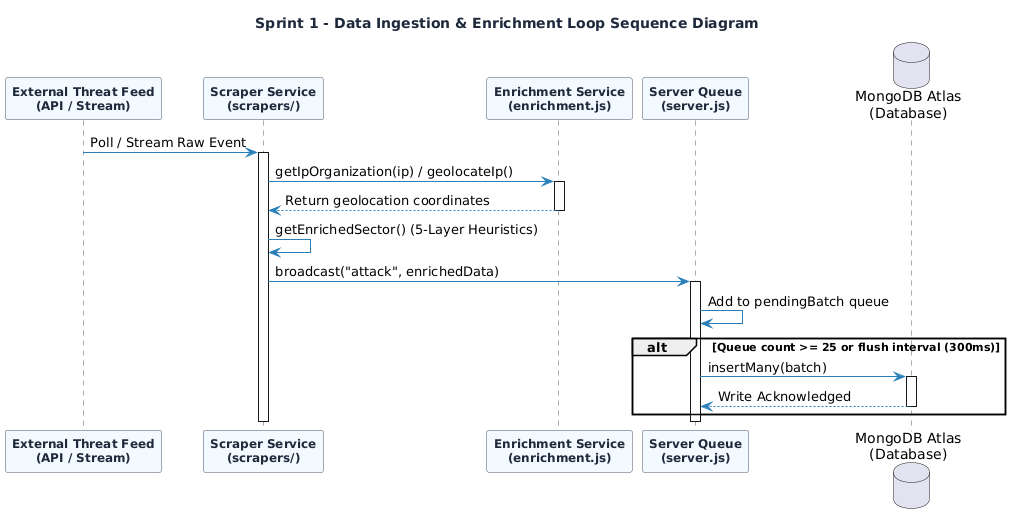
\includegraphics[width=0.95\textwidth]{assets/s1_sequence.png}
\caption{Sprint 1: Sequence diagram of the harvesting and enrichment loop.}
\label{fig:s1_sequence}
\end{figure}

---

\subsection{Sprint Realization: Detailed Scraper Implementations}
The harvesters are located in \texttt{backend/services/scrapers/}. To ensure complete operational isolation, thread resilience, and modular error recovery, we implemented a decoupled execution model. The core Express orchestrator (\texttt{server.js}) dynamically registers each scraper module, executing their ingestion loops within separate asynchronous promise contexts. This ensures that if a single external feed encounters network timeouts, rate-limit blocks, or malformed responses, the remaining scrapers continue to operate.

Below, we catalog and detail the architectural specifications, raw payload schemas, and normalization pipelines for each of the 9 integrated cyber threat intelligence harvesters.

\subsubsection{1. Checkpoint Scraper (\texttt{checkpoint.js})}
\begin{itemize}
    \item \textbf{Source Endpoint \& Protocol:} Establishes a direct, long-lived, secure Server-Sent Events (SSE) HTTP stream connection to Checkpoint's corporate live threat telemetry server (summarized in Table~\ref{tab:spec_checkpoint}).
    \begin{table}[htbp]
    \centering
    \small
    \begin{tabular}{ll}
    \toprule
    \textbf{Specification Parameter} & \textbf{Configuration Value} \\
    \midrule
    Protocol & HTTP/1.1 Server-Sent Events (SSE) \\
    Endpoint URL & \url{https://threatmap.checkpoint.com/feed/live} \\
    Transport Security & TLS 1.3 Encryption \\
    Connection Mode & Active Persistent Client Stream \\
    \bottomrule
    \end{tabular}
    \caption{Checkpoint Scraper Endpoint Specifications.}
    \label{tab:spec_checkpoint}
    \end{table}

    \item \textbf{Expected Payload Schema:} The stream broadcasts newline-separated SSE threat packets. The parsed JSON data attributes are defined in Table~\ref{tab:payload_checkpoint} (with the raw payload example detailed in Appendix I.1).
    \begin{table}[htbp]
    \centering
    \small
    \begin{tabular}{lll}
    \toprule
    \textbf{JSON Attribute} & \textbf{Data Type} & \textbf{Description / Constraints} \\
    \midrule
    \texttt{srcIp} & String & Source IPv4 or IPv6 Address \\
    \texttt{dstIp} & String & Target/Destination IP Address \\
    \texttt{attackName} & String & Exploit name or signature identifier \\
    \texttt{attackType} & String & Threat class category (e.g. \texttt{phishing}) \\
    \texttt{severity} & String & Threat severity level string \\
    \texttt{srcCountry} & String & Origin ISO two-letter country code \\
    \texttt{dstCountry} & String & Target ISO two-letter country code \\
    \bottomrule
    \end{tabular}
    \caption{Checkpoint Raw Threat Payload Schema.}
    \label{tab:payload_checkpoint}
    \end{table}

    \item \textbf{Operation Mechanism:} The scraper operates as an active, persistent client listener. Upon establishing the socket, it parses incoming chunks line-by-line, validating that the packet contains valid \texttt{srcIp} and \texttt{dstIp} parameters.
    \item \textbf{Data Normalization \& Error Handling:} Evaluates incoming event keys and maps them directly into our BSON schema. Phishing indicators are routed to the \texttt{phishing} category. If Checkpoint's stream is disconnected, the module initiates an automated reconnect routine with a 5-second backoff delay, logging a warning to the central controller.
\end{itemize}

\subsubsection{2. Bitdefender Live Telemetry Scraper (\texttt{bitdefender.js})}
\begin{itemize}
    \item \textbf{Source Endpoint \& Protocol:} Establishes a real-time Web Socket connection using the \texttt{socket.io-client} protocol to Bitdefender's global threat intelligence sharing hub (summarized in Table~\ref{tab:spec_bitdefender}).
    \begin{table}[htbp]
    \centering
    \small
    \begin{tabular}{ll}
    \toprule
    \textbf{Specification Parameter} & \textbf{Configuration Value} \\
    \midrule
    Protocol & WebSocket (socket.io Transport) \\
    Endpoint URL & \url{wss://hub.bitdefender.com/threat-telemetry} \\
    Active Channels & 13 Threat Channels (e.g. ransomware, botnet) \\
    Connection Mode & Bidirectional Event Socket \\
    \bottomrule
    \end{tabular}
    \caption{Bitdefender Scraper Endpoint Specifications.}
    \label{tab:spec_bitdefender}
    \end{table}

    \item \textbf{Expected Payload Schema:} The WebSocket channel broadcasts binary frames converted into JSON. The attributes are listed in Table~\ref{tab:payload_bitdefender} (with the raw payload example detailed in Appendix I.2).
    \begin{table}[htbp]
    \centering
    \small
    \begin{tabular}{lll}
    \toprule
    \textbf{JSON Attribute} & \textbf{Data Type} & \textbf{Description / Constraints} \\
    \midrule
    \texttt{event} & String & Event action classifier (e.g. \texttt{detection}) \\
    \texttt{channel} & String & Source channel name mapped to threat vector \\
    \texttt{ip} & String & Intercepted source IP address string \\
    \texttt{country} & String & Origin country code (ISO Alpha-2) \\
    \texttt{malwareName} & String & Specific malware signature family name \\
    \texttt{port} & Number & Target connection port (used for sector mapping) \\
    \bottomrule
    \end{tabular}
    \caption{Bitdefender Raw Threat Payload Schema.}
    \label{tab:payload_bitdefender}
    \end{table}

    \item \textbf{Operation Mechanism:} Subscribes to 13 distinct active channels representing diverse attack vectors (e.g. ransomware, malicious URLs, botnets). The socket interface receives live notifications.
    \item \textbf{Data Normalization:} The channel name determines the target threat class mapping. If the event is received on the \texttt{ransomware} channel, the scraper sets \texttt{a\_t = "malware"} and maps the target sector using port-based heuristics (port 445 maps to "Enterprise Technology").
\end{itemize}

\subsubsection{3. Fortinet FortiGuard Scraper (\texttt{fortinet.js})}
\begin{itemize}
    \item \textbf{Source Endpoint \& Protocol:} Polls Fortinet's active exploit telemetry API using standard stateless HTTP queries (summarized in Table~\ref{tab:spec_fortinet}).
    \begin{table}[htbp]
    \centering
    \small
    \begin{tabular}{ll}
    \toprule
    \textbf{Specification Parameter} & \textbf{Configuration Value} \\
    \midrule
    Protocol & HTTP/1.1 REST API (GET) \\
    Endpoint URL & \url{https://fortiguard.com/api/threats/active} \\
    Custom Headers & \texttt{User-Agent: Predictra-Ingestion-Agent/1.0} \\
    Polling Frequency & Every 4 seconds \\
    \bottomrule
    \end{tabular}
    \caption{Fortinet Scraper Endpoint Specifications.}
    \label{tab:spec_fortinet}
    \end{table}

    \item \textbf{Expected Payload Schema:} The API returns a structured JSON array of exploit records. The schema fields are defined in Table~\ref{tab:payload_fortinet} (with the raw payload example detailed in Appendix I.3).
    \begin{table}[htbp]
    \centering
    \small
    \begin{tabular}{lll}
    \toprule
    \textbf{JSON Attribute} & \textbf{Data Type} & \textbf{Description / Constraints} \\
    \midrule
    \texttt{srcCountry} & String & Full country name of attacker origin \\
    \texttt{dstCountry} & String & Full country name of victim target \\
    \texttt{signatureName} & String & Specific exploit name (e.g. Apache Log4j) \\
    \texttt{attackCount} & Number & Aggregated count of attack occurrences \\
    \texttt{victimSubnet} & String & Masked network subnet of victim \\
    \bottomrule
    \end{tabular}
    \caption{Fortinet Raw Threat Payload Schema.}
    \label{tab:payload_fortinet}
    \end{table}

    \item \textbf{Operation Mechanism:} Evaluates recent active exploit campaigns on a 4-second polling schedule. The scraper iterates through the returned array, parses the country strings into ISO two-letter country codes (e.g. "Germany" to "DE"), and extracts the attack name.
    \item \textbf{Data Normalization:} Since Fortinet records reflect active intrusion attempts, threat events are registered under \texttt{a\_t = "exploit"}, and \texttt{a\_c} is mapped directly to the \texttt{attackCount} parameter.
\end{itemize}

\subsubsection{4. URLhaus Malware Scraper (\texttt{urlhaus.js})}
\begin{itemize}
    \item \textbf{Source Endpoint \& Protocol:} Queries abuse.ch's URLhaus API to retrieve newly identified malicious URL distribution nodes (summarized in Table~\ref{tab:spec_urlhaus}).
    \begin{table}[htbp]
    \centering
    \small
    \begin{tabular}{ll}
    \toprule
    \textbf{Specification Parameter} & \textbf{Configuration Value} \\
    \midrule
    Protocol & HTTP/1.1 REST API (POST) \\
    Endpoint URL & \url{https://urlhaus-api.abuse.ch/v1/urls/recent/} \\
    Polling Frequency & Every 90 seconds \\
    \bottomrule
    \end{tabular}
    \caption{URLhaus Scraper Endpoint Specifications.}
    \label{tab:spec_urlhaus}
    \end{table}

    \item \textbf{Expected Payload Schema:} Returns a dictionary containing a list of active threat URLs. The schema fields for each item are defined in Table~\ref{tab:payload_urlhaus} (with the raw payload example detailed in Appendix I.4).
    \begin{table}[htbp]
    \centering
    \small
    \begin{tabular}{lll}
    \toprule
    \textbf{JSON Attribute} & \textbf{Data Type} & \textbf{Description / Constraints} \\
    \midrule
    \texttt{id} & String & Unique integer identifier for URL block \\
    \texttt{url} & String & Full HTTP/HTTPS address serving malware payload \\
    \texttt{url\_status} & String & Online/offline reachability flag \\
    \texttt{threat} & String & Threat class label (e.g. \texttt{malware\_download}) \\
    \texttt{reporter} & String & Name of threat researcher or bot submitter \\
    \texttt{tags} & Array & Threat signature list tags (e.g. CobaltStrike) \\
    \bottomrule
    \end{tabular}
    \caption{URLhaus Raw Threat Payload Schema.}
    \label{tab:payload_urlhaus}
    \end{table}

    \item \textbf{Operation Mechanism:} The scraper parses the \texttt{urls} list, filtering for entries where \texttt{url\_status} is \texttt{"online"}. It uses regex queries to isolate the IP address or domain name from the raw \texttt{url} string (e.g., extracting \texttt{"185.220.101.5"} as the source IP).
    \item \textbf{Data Normalization:} Since these represent active malware distribution files, all events are registered under \texttt{a\_t = "malware"}. The first entry in the \texttt{tags} array is assigned to \texttt{a\_n}.
\end{itemize}

\subsubsection{5. Kaspersky Feodo Botnet Tracker (\texttt{kaspersky.js})}
\begin{itemize}
    \item \textbf{Source Endpoint \& Protocol:} Polls abuse.ch's Feodo Tracker database of active Botnet command-and-control (C2) servers (summarized in Table~\ref{tab:spec_kaspersky}).
    \begin{table}[htbp]
    \centering
    \small
    \begin{tabular}{ll}
    \toprule
    \textbf{Specification Parameter} & \textbf{Configuration Value} \\
    \midrule
    Protocol & HTTP/1.1 REST (GET) \\
    Endpoint URL & \url{https://feodotracker.abuse.ch/downloads/ipblocklist.csv} \\
    Polling Frequency & Every 60 seconds \\
    \bottomrule
    \end{tabular}
    \caption{Kaspersky Feodo Scraper Endpoint Specifications.}
    \label{tab:spec_kaspersky}
    \end{table}

    \item \textbf{Expected Payload Schema:} The feed returns CSV formatted text lines. The schema fields mapping to the CSV headers are defined in Table~\ref{tab:payload_kaspersky} (with the raw payload example detailed in Appendix I.5).
    \begin{table}[htbp]
    \centering
    \small
    \begin{tabular}{lll}
    \toprule
    \textbf{CSV Attribute} & \textbf{Data Type} & \textbf{Description / Constraints} \\
    \midrule
    \texttt{Firstseen} & Date String & Date/time the node was first registered \\
    \texttt{DstIP} & String & Destination Command \& Control IP address \\
    \texttt{DstPort} & Number & Listening port of the C2 framework \\
    \texttt{Malware} & String & Name of active botnet malware (e.g. Qakbot) \\
    \texttt{Asname} & String & Autonomous System (AS) network ISP name \\
    \bottomrule
    \end{tabular}
    \caption{Kaspersky Feodo Raw Threat Payload Schema.}
    \label{tab:payload_kaspersky}
    \end{table}

    \item \textbf{Operation Mechanism:} The scraper retrieves the CSV string, splits it by newline characters, ignores comment lines, and splits each data line by commas. It extracts the destination IP (\texttt{DstIP}), destination port (\texttt{DstPort}), and the specific malware family (\texttt{Malware}).
    \item \textbf{Data Normalization:} Botnet controller nodes are mapped to \texttt{a\_t = "malware"}. The source IP is assigned to \texttt{DstIP}, and target sectors are mapped based on the listening port (port 443 defaults to "Enterprise Services").
\end{itemize}

\subsubsection{6. AlienVault OTX Pulse Scraper (\texttt{alienvault.js})}
\begin{itemize}
    \item \textbf{Source Endpoint \& Protocol:} Queries the AlienVault Open Threat Exchange REST API, utilizing custom developer API authentication tokens (summarized in Table~\ref{tab:spec_alienvault}).
    \begin{table}[htbp]
    \centering
    \small
    \begin{tabular}{ll}
    \toprule
    \textbf{Specification Parameter} & \textbf{Configuration Value} \\
    \midrule
    Protocol & HTTP/1.1 REST (GET) \\
    Endpoint URL & \url{https://otx.alienvault.com/api/v1/pulses/subscribed} \\
    Custom Headers & \texttt{X-OTX-API-KEY: <custom\_otx\_api\_token>} \\
    Polling Frequency & Every 5 minutes \\
    \bottomrule
    \end{tabular}
    \caption{AlienVault Scraper Endpoint Specifications.}
    \label{tab:spec_alienvault}
    \end{table}

    \item \textbf{Expected Payload Schema:} Returns nested threat pulses. The parsed schema attributes are described in Table~\ref{tab:payload_alienvault} (with the raw payload example detailed in Appendix I.6).
    \begin{table}[htbp]
    \centering
    \small
    \begin{tabular}{lll}
    \toprule
    \textbf{JSON Attribute} & \textbf{Data Type} & \textbf{Description / Constraints} \\
    \midrule
    \texttt{count} & Number & Count of pulse objects returned in response \\
    \texttt{name} & String & Threat intelligence pulse campaign name \\
    \texttt{description} & String & Text summary details of adversary activities \\
    \texttt{indicator} & String & Specific indicator string (IP address or hash) \\
    \texttt{type} & String & IOC type tag indicator (e.g. \texttt{IPv4}, \texttt{FileHash}) \\
    \bottomrule
    \end{tabular}
    \caption{AlienVault Raw Threat Payload Schema.}
    \label{tab:payload_alienvault}
    \end{table}

    \item \textbf{Operation Mechanism:} Polls every 5 minutes, pulling recent indicators of compromise (IOC) from subscribed threat pulses. It parses IP addresses, hashes, and vulnerability details.
    \item \textbf{Data Normalization:} The scraper iterates through the nested \texttt{indicators} array. Only indicators of type \texttt{IPv4} are geolocated. The threat name \texttt{a\_n} is derived from the main pulse \texttt{name}.
\end{itemize}

\subsubsection{7. Ransomwatch Extortion Scraper (\texttt{ransomwatch.js})}
\begin{itemize}
    \item \textbf{Source Endpoint \& Protocol:} Polls the Ransomlook.io API endpoint monitoring active ransomware extortion leak sites (summarized in Table~\ref{tab:spec_ransomwatch}).
    \begin{table}[htbp]
    \centering
    \small
    \begin{tabular}{ll}
    \toprule
    \textbf{Specification Parameter} & \textbf{Configuration Value} \\
    \midrule
    Protocol & HTTP/1.1 REST (GET) \\
    Endpoint URL & \url{https://ransomlook.io/api/posts/recent} \\
    Polling Frequency & Every 10 minutes \\
    \bottomrule
    \end{tabular}
    \caption{Ransomwatch Scraper Endpoint Specifications.}
    \label{tab:spec_ransomwatch}
    \end{table}

    \item \textbf{Expected Payload Schema:} Returns a list of dark web leak site posts. The metadata attributes are defined in Table~\ref{tab:payload_ransomwatch} (with the raw payload example detailed in Appendix I.7).
    \begin{table}[htbp]
    \centering
    \small
    \begin{tabular}{lll}
    \toprule
    \textbf{JSON Attribute} & \textbf{Data Type} & \textbf{Description / Constraints} \\
    \midrule
    \texttt{group} & String & Name of ransomware developer group (e.g. LockBit) \\
    \texttt{post\_title} & String & Title containing victim corporation name string \\
    \texttt{discovered} & Date String & Timestamp when post was first indexed \\
    \texttt{website} & String & Darknet onion address of the extortion site \\
    \bottomrule
    \end{tabular}
    \caption{Ransomwatch Raw Threat Payload Schema.}
    \label{tab:payload_ransomwatch}
    \end{table}

    \item \textbf{Operation Mechanism:} Ransomware attacks target organizations rather than specific IP addresses. When a new post is parsed, the scraper extracts the victim name from \texttt{post\_title} ("Texas Medical Center Inc"). It geolocates the victim based on target location keywords ("Texas" to United States coordinates).
    \item \textbf{Data Normalization:} All events are registered as ransomware indicators under \texttt{a\_t = "malware"}. The target business sector is resolved using our 5-layer classification engine (matching "Medical" to "Healthcare").
\end{itemize}

\subsubsection{8. MontySecurity C2 Tracker (\texttt{c2tracker.js})}
\begin{itemize}
    \item \textbf{Source Endpoint \& Protocol:} Polls the MontySecurity command-and-control tracker endpoint to monitor active listener framework IPs (summarized in Table~\ref{tab:spec_c2tracker}).
    \begin{table}[htbp]
    \centering
    \small
    \begin{tabular}{ll}
    \toprule
    \textbf{Specification Parameter} & \textbf{Configuration Value} \\
    \midrule
    Protocol & HTTP/1.1 REST (GET) \\
    Endpoint URL & \url{https://github.com/c2/active/c2.json} \\
    Polling Frequency & Every 15 minutes \\
    \bottomrule
    \end{tabular}
    \caption{MontySecurity C2 Scraper Endpoint Specifications.}
    \label{tab:spec_c2tracker}
    \end{table}

    \item \textbf{Expected Payload Schema:} Returns active command host framework arrays. The JSON fields are described in Table~\ref{tab:payload_c2tracker} (with the raw payload example detailed in Appendix I.8).
    \begin{table}[htbp]
    \centering
    \small
    \begin{tabular}{lll}
    \toprule
    \textbf{JSON Attribute} & \textbf{Data Type} & \textbf{Description / Constraints} \\
    \midrule
    \texttt{ip} & String & Public IP address of the listening C2 server \\
    \texttt{framework} & String & C2 framework software name (e.g. Cobalt Strike) \\
    \texttt{port} & Number & Server listening port number \\
    \texttt{first\_seen} & String & Date string of initial detection \\
    \bottomrule
    \end{tabular}
    \caption{MontySecurity C2 Raw Threat Payload Schema.}
    \label{tab:payload_c2tracker}
    \end{table}

    \item \textbf{Operation Mechanism:} The scraper parses active C2 servers. The parser extracts host IPs, listening ports, and malware families (e.g. Cobalt Strike, Mythic).
    \item \textbf{Data Normalization:} Since these servers control bots, threat events map to \texttt{a\_t = "malware"}. The indicator name is formatted as \texttt{a\_n = "Cobalt Strike C2 Node"}.
\end{itemize}

\subsubsection{9. MISP Galaxy Synthetic Scraper (\texttt{misp-galaxy.js})}
\begin{itemize}
    \item \textbf{Source Endpoint \& Protocol:} Accesses local JSON data structures cached inside the backend configuration folder (summarized in Table~\ref{tab:spec_misp_galaxy}).
    \begin{table}[htbp]
    \centering
    \small
    \begin{tabular}{ll}
    \toprule
    \textbf{Specification Parameter} & \textbf{Configuration Value} \\
    \midrule
    Protocol & Local In-Memory JSON Parsing (File Read) \\
    Cache Directory & \texttt{backend/config/misp-galaxy/} \\
    Refresh Interval & Every 6 hours \\
    Synthetic Emission & Random interval of 20 seconds \\
    \bottomrule
    \end{tabular}
    \caption{MISP Galaxy Scraper Endpoint Specifications.}
    \label{tab:spec_misp_galaxy}
    \end{table}

    \item \textbf{Expected Payload Schema:} Evaluates cached MISP JSON metadata templates. The main template structures are defined in Table~\ref{tab:payload_misp_galaxy} (with the raw payload format referenced in Appendix I.9).
    \begin{table}[htbp]
    \centering
    \small
    \begin{tabular}{lll}
    \toprule
    \textbf{JSON Attribute} & \textbf{Data Type} & \textbf{Description / Constraints} \\
    \midrule
    \texttt{galaxy} & String & Galaxy class name identifier (e.g. threat-actor) \\
    \texttt{name} & String & Name of the threat actor cluster or malware family \\
    \texttt{description} & String & Detailed narrative of target profiling and CVEs \\
    \texttt{uuid} & String & Unique OASIS STIX-compliant entity UUID \\
    \bottomrule
    \end{tabular}
    \caption{MISP Galaxy Raw Threat Payload Schema.}
    \label{tab:payload_misp_galaxy}
    \end{table}

    \item \textbf{Operation Mechanism:} Caches massive threat actor clusters and malware family metadata locally every 6 hours, emitting geocoded synthetic events every 20 seconds to populate visual screens.
    \item \textbf{Data Normalization:} Derives attributes from MISP actor and target metadata files.
\end{itemize}

---

\subsection{Sprint Realization: Ingestion \& Enrichment Logic}

\subsubsection{Enrichment Logic Walkthrough}
The enrichment file `backend/services/enrichment.js` contains a robust **5-Layer Sector Classification Engine** designed to identify target organization domains:
\begin{enumerate}
    \item \textbf{Victim Name Keywords:} Performs word-boundary matching on \texttt{d\_ip} organization details against custom dictionaries of critical sectors (e.g., matching "Ministry" to "Government").
    \item \textbf{Event Details Keywords:} Runs regex matches on the malware name or event description.
    \item \textbf{Port-Based Mapping:} Maps common attack ports (e.g., port 445/139 to "Enterprise Technology", 3306/1521 to "Databases/Retail", 5060 to "Telecom").
    \item \textbf{MISP Galaxy Metadata:} Directly parses targeting tags from the cached MISP dataset.
    \item \textbf{Source API Fallback:} Uses default sector mappings aligned with the scraper's nature (e.g., `ransomwatch.js` defaults to "Finance / Business").
\end{enumerate}

To enrich the geolocated organizational contexts, we also implemented an **asynchronous RDAP (Registration Data Access Protocol) query** with a 3-second timeout and an in-memory organization cache to resolve IP address owners without adding loop latency.

\subsubsection{Sprint Interfaces and Console Verification}
\begin{itemize}
    \item \textbf{Scraper Log Console:} The backend logs show active polling actions:
    \begin{verbatim}
    [Bitdefender] connected. Subscribed to 13 threat feeds channels.
    [Fortinet] Ingested 45 threat logs. Geocoded and broadcasted.
    [MongoDB] Bulk insert successfully flushed 25 threat documents.
    \end{verbatim}
    \item \textbf{Persistence Test:} We verified MongoDB collections using Compass, confirming that all compact fields (\texttt{a\_n}, \texttt{s\_la}, \texttt{source\_api}) mapped correctly with 30-day index expirations active.
\end{itemize}

---

\section{Sprint 2: Real-Time SSE Stream and 3D Globe Visualization}

\subsection{Sprint Backlog and Objectives}
Sprint 2 covered the frontend and communication setup. The goal was to write the Express Server-Sent Events (SSE) broadcast endpoint, establish the Zustand store client, build the interactive 3D WebGL Earth canvas with React Three Fiber, and render elevated bezier arcs and expanding markers.

\subsection{Sprint Analysis: Use Case Modeling}
The visualizer use cases are captured in Figure~\ref{fig:s2_usecase}, illustrating the analyst's dashboard controls.

\begin{figure}[htbp]
\centering
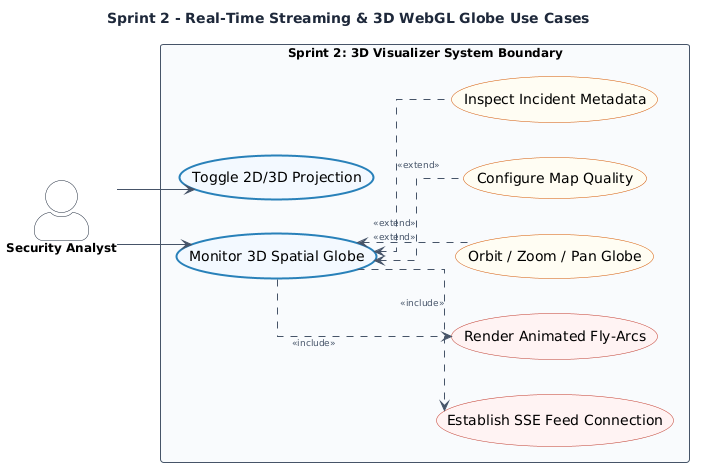
\includegraphics[width=0.95\textwidth]{assets/s2_usecase.png}
\caption{Sprint 2: Use Case diagram for the 3D map visualizer.}
\label{fig:s2_usecase}
\end{figure}

The functional steps are detailed in Table~\ref{tab:s2_uc_desc}.

\begin{table}[htbp]
\centering
\small
\begin{tabular}{>{\raggedright\arraybackslash}p{2.8cm}>{\raggedright\arraybackslash}p{5.2cm}>{\raggedright\arraybackslash}p{5.2cm}}
\toprule
\textbf{Use Case} & \textbf{Actor/Trigger} & \textbf{Main Workflow} \\
\midrule
Monitor 3D Spatial Globe & Security Analyst / Mounts Page & Connects the client browser to the live `/api/feed` stream. Incoming events are geocoded to 3D vectors and drawn as animated great-circle arcs and pulsating circles. \\
Toggle 2D Projection & Security Analyst / Clicks HUD Button & Triggers a coordinate system interpolation, flattening the Three.js mesh spheres into a flat 2D Mercator layout. \\
\bottomrule
\end{tabular}
\caption{Sprint 2: Use Case descriptions.}
\label{tab:s2_uc_desc}
\end{table}

\subsection{Sprint Conception: Trigonometric Geocoding and Arc Interpolation}
Building a high-performance 3D visual mapping environment requires a solid mathematical foundation. To bridge the gap between geographical databases (which express threat locations using standard Latitude/Longitude coordinate systems) and WebGL canvases (which require 3D spatial vector arrays), we designed custom geocoding and curve-generation pipelines.

\subsubsection{Spatial Projection Mathematics (Latitude/Longitude to Vector3)}
To project geolocated coordinates onto the procedural Three.js sphere, the system translates geographic coordinates (standard latitude and longitude values in degrees) into three-dimensional Cartesian vector coordinates. This mapping operates within a coordinate system relative to a sphere of a predefined radius (typically set to a base unit of 1.0).

First, the geographic angles in degrees are mathematically scaled into radians. To ensure the rendered map projection aligns perfectly with the WebGL screen orientation, the longitude is offset by 180 degrees before scaling, and the latitude is directly converted. The system then computes the Cartesian coordinates. The horizontal coordinate (X-axis) is defined as the negative product of the sphere radius, the cosine of the radian latitude, and the cosine of the radian longitude. The vertical coordinate (Y-axis) is defined as the product of the sphere radius and the sine of the radian latitude. Finally, the depth coordinate (Z-axis) is defined as the product of the sphere radius, the cosine of the radian latitude, and the sine of the radian longitude.

The inclusion of the negative sign on the horizontal projection (X-axis) is a critical requirement of the WebGL rendering context. Three.js utilizes a right-handed coordinate system where the positive Z-axis points directly outward from the screen, the positive Y-axis points upwards, and the positive X-axis points rightwards. Omitting this directional inversion would cause the geocoded map coordinates to mirror horizontally, placing geographical boundaries in the incorrect hemispheres.

\subsubsection{Trigonometric Derivation of Spherical Linear Interpolation (SLERP)}
To render an attack arc flying out from a source coordinates vector to a destination coordinates vector across the sphere surface, a simple linear interpolation of coordinates is geometrically incorrect. A linear interpolation (LERP) would cut straight through the three-dimensional volume of the sphere, resulting in a straight line that sinks directly beneath the curved surface mesh of the Earth.

To ensure that the attack trail flies gracefully along the curved surface of the globe, the system utilizes Spherical Linear Interpolation (SLERP). The algorithm first calculates the angular separation between the two unit position vectors (the source vector and the destination vector). This is achieved by taking the vector dot product of the two coordinates, which represents the cosine of the separation angle.

Using this angular separation, the intermediate coordinates are interpolated along the curved surface for any progress state (ranging from zero percent at the start to one hundred percent at the destination). The algorithm scales each of the two terminal vectors using sine-based ratios of the progress state and the total angular separation. This specific sine-based weighting ensures a constant angular velocity across the entire flight path. As a result, the particle trails move at a perfectly uniform speed, avoiding unrealistic accelerations or deceleration spikes near the starting or ending coordinates.

\subsubsection{Parametric Quadratic Bezier Fly-Arcs}
While spherical linear interpolation keeps paths aligned to the sphere's surface, rendering multiple overlapping tracks directly on the globe makes visual analysis difficult. To represent attack vectors as elevated volumetric fibers, the arcs are designed to rise radially outward, reaching their peak altitude exactly at the midpoint of their flight trajectory:
\begin{enumerate}
    \item The system first computes a surface midpoint coordinates vector. This is done by performing a spherical linear interpolation between the source and destination vectors at exactly fifty percent of the flight progress.
    \item An elevated control point vector is then projected radially outward from the center of the sphere. This is achieved by scaling the surface midpoint vector by an elevation multiplier. This multiplier is calculated by adding a base scale factor to the product of a dynamic arc height scalar coefficient (typically set between 0.25 and 0.45) and the angular distance between the source and destination vectors. This dynamic scaling guarantees that long-distance intercontinental attacks arch significantly higher into space, while local regional queries remain low and close to the surface, visually sorting the severity and scope of threat streams.
    \item These three coordinate vectors (the source vector, the elevated control vector, and the destination vector) are passed to the Three.js quadratic Bezier curve constructor. The resulting curve is evaluated parametrically using quadratic Bernstein polynomials to generate a smooth, continuous path. This path starts at the origin coordinates, reaches its maximum radial height in outer space at the midpoint, and sweeps down to the target coordinates, providing a beautiful neon volumetric path.
\end{enumerate}

\subsubsection{UML Sequence Diagram}
The real-time streaming pipeline from scraper broadcasts to frontend Zustand store accumulation and WebGL rendering cycles is traced in Figure~\ref{fig:s2_sequence}.

\begin{figure}[htbp]
\centering
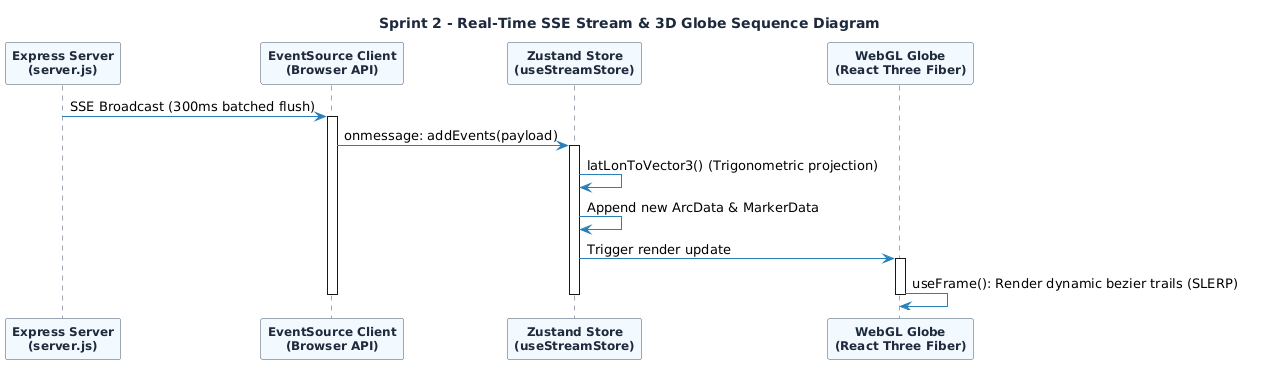
\includegraphics[width=0.95\textwidth]{assets/s2_sequence.png}
\caption{Sprint 2: Sequence diagram of real-time streaming and WebGL rendering.}
\label{fig:s2_sequence}
\end{figure}

---

\subsection{Sprint Realization: Shaders, Shards, and WebGL Globe}

\subsubsection{Server-Sent Events (SSE) Broadcast Engine}
Rather than using heavy WebSockets, we built an optimized SSE route \texttt{GET /api/feed} in \texttt{backend/server.js}:
\begin{itemize}
    \item Sets the required streaming headers: \texttt{Content-Type} (set to \texttt{text/}\allowbreak\texttt{event-stream}), \texttt{Cache-Control} (set to \texttt{no-cache}), and \texttt{Connection} (set to \texttt{keep-alive}).
    \item Incoming scrapers immediately queue threat events into a memory array.
    \item The server runs a \textbf{300ms flush interval scheduler}, consolidating all queued events into a single payload array and writing it to connected clients. This avoids browser rendering lockups from rapid single-event updates.
    \item A \textbf{30-second ping heartbeat} is emitted to keep connections open through proxies.
\end{itemize}

\subsubsection{3D Earth Shader Realization}
Our primary globe mesh in \texttt{globe/Earth.tsx} implements a highly performant, custom-shaded sphere:
\begin{itemize}
    \item \textbf{Custom GLSL Shaders:} To create a premium visual experience, the globe mesh avoids standard flat image textures. Instead, we wrote custom WebGL vertex and fragment shaders using OpenGL Shading Language (GLSL). The vertex shader passes surface normals to the fragment shader, which computes a real-time \textbf{Fresnel atmospheric glow} based on the relationship between the surface normal vector and the camera's line-of-sight view vector. Specifically, the shader calculates the vector dot product of the surface normal and the camera view direction, restricts this value to a non-negative range, subtracts it from a maximum intensity unit, and raises the result to a power falloff factor (typically set to a factor of 4.0). This creates a high-fidelity glowing border around the outer silhouette of the globe that fades smoothly towards the center.
    
    To illustrate this shader logic, Table~\ref{tab:glow_shader_vars} outlines the shader attributes and parameters passed between the rendering passes, with the complete source code detailed in Appendix H.1:

    \begin{table}[htbp]
    \centering
    \small
    \begin{tabular}{lll}
    \toprule
    \textbf{Variable Name} & \textbf{GLSL Type} & \textbf{Role / Computational Purpose} \\
    \midrule
    \texttt{vNormal} & \texttt{varying vec3} & Surface normal vector passed from vertex to fragment shader \\
    \texttt{normalMatrix} & \texttt{uniform mat3} & Standard WebGL transformation matrix mapping normals \\
    \texttt{mvPosition} & \texttt{vec4} & Model-View matrix mapping physical coordinates on sphere \\
    \texttt{dotProd} & \texttt{float} & Dot product measuring normal cosine angle relative to camera \\
    \texttt{intensity} & \texttt{float} & Power-scaled intensity falloff function for Fresnel scattering \\
    \texttt{atmosphericColor} & \texttt{vec3} & Neon Cyberblue color vector (\texttt{0.23, 0.51, 0.96}) \\
    \texttt{gl\_FragColor} & \texttt{vec4} & Output pixel color vector containing transparency blending \\
    \bottomrule
    \end{tabular}
    \caption{Atmospheric Glow Shader Parameters and Interpolated Variables.}
    \label{tab:glow_shader_vars}
    \end{table}
    
    \item \textbf{TopoJSON Country Outlines:} Loads a lightweight TopoJSON land coordinate file (\texttt{land-110m.json}) and projects the land boundaries as vector lines.
    \item \textbf{Neon Glow Borders:} Renders country borders using \textbf{5 overlapping vector line layers} at microscopic scale increases (from $R=1.002$ to $R=1.010$) with decreasing opacities, creating a beautiful neon outline glow effect without needing heavy blur shaders.
    \item \textbf{Post-Processing Bloom:} Wraps the R3F \texttt{<Canvas>} in \texttt{<EffectComposer>}, using a high-fidelity \texttt{<Bloom>} shader (luminanceThreshold 0.15, intensity 0.8) to make severity-colored attack arcs glow like neon light fibers.
\end{itemize}

---

\section{Conclusion}
This chapter detailed the completion of our first main release. By combining a parallel harvester backend with geocoders and establishing the 300ms SSE broadcast channel, we successfully rendered the 3D procedural WebGL threat globe at 60fps, displaying active threat events as volumetric glowing bezier arcs. We proceed to Chapter 4 to document the second release, detailing the analytical STIX 2.1 graph, historical browser, and performance guardrails.

\chapter{Second Release - STIX Analytics and Performance Guardrails}

\section{Introduction}
This chapter presents the design, Unified Modeling Language (UML) modeling, and advanced technical implementation of the second functional release of the platform, matching the \textbf{Release 2} specifications of the Predictra CTI system. This release covers \textbf{Sprint 3 (STIX 2.1 Threat Analysis Dashboard)} and \textbf{Sprint 4 (Analytics, History, and Performance Polishing)}. 

For each sprint, we deeply analyze the backlog objectives, describe functional system boundaries via UML Use Case modeling, detail the structural class layouts and transactional sequences, provide the mathematical foundations of graph physics and memory buffer allocations, walk through the actual React/TypeScript code logic, and illustrate the realized interfaces. This chapter represents the high-performance and analytical layer of the Predictra Threat Map, ensuring that visual alerts are paired with standard-compliant cyber threat intelligence.

\section{Sprint 3: STIX 2.1 Threat Analysis Dashboard}

\subsection{Sprint Backlog and Objectives}
The primary objective of Sprint 3 was to equip the platform with deep, standardized analytical capabilities. While a real-time visual map is excellent for immediate situational awareness, security investigators require structured frameworks to trace complex campaigns. To fulfill this need, we implemented support for the \textbf{Structured Threat Information Expression (STIX) Version 2.1} standard, which is an XML/JSON-based serialization format developed by OASIS to represent cyber threat intelligence.

The Sprint 3 backlog focused on two key deliverables:
\begin{itemize}
    \item \textbf{STIX 2.1 JSON Ingestion Service:} A client-side file upload and validation component to parse large, multi-megabyte intelligence bundles without overloading browser processes.
    \item \textbf{MITRE ATT\&CK Cyber Kill Chain Mapping Grid:} An automated taxonomy engine that maps ingested adversary behaviors directly to the 12 classic phases of the MITRE enterprise attack grid.
\end{itemize}

\subsection{Sprint Analysis: Use Case Modeling}
The analyst's interactions with the STIX workspace are captured in Figure~\ref{fig:s3_usecase} using a Use Case diagram, illustrating actor boundaries and system triggers.

\begin{figure}[H]
\centering
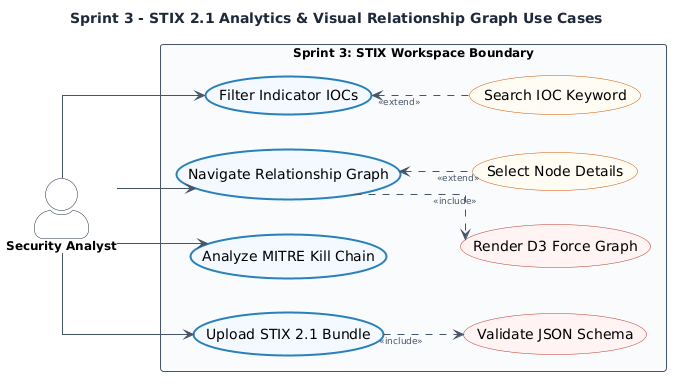
\includegraphics[width=0.95\textwidth]{assets/s3_usecase.png}
\caption{Sprint 3: Use Case diagram for the STIX 2.1 dashboard.}
\label{fig:s3_usecase}
\end{figure}

The functional workflows and validation rules for each use case are documented in Table~\ref{tab:s3_uc_desc_expanded}.

\begin{table}[H]
\centering
\small
\arrayrulecolor{charcoal!30}
\rowcolors{2}{cyberblue!5}{white}
\begin{tabularx}{\textwidth}{>{\raggedright\arraybackslash}p{2.6cm}>{\raggedright\arraybackslash}p{4.4cm}X}
\hline
\rowcolor{charcoal}
\thc{Use Case} & \thc{Actor/Trigger} & \thc{Main Workflow \& Validation Rules} \\
\hline
Upload STIX 2.1 & Security Analyst / Uploads JSON File & 1. Analyst uploads a STIX JSON file. \\
 & & 2. The parser validates the existence of the `type: "bundle"` attribute and reads the JSON structures. \\
 & & 3. If validation fails, an error toast is displayed. \\
\hline
Filter IOCs & Security Analyst / Types in Search & 1. Analyst filters by search text or select box (IP, Hash, URL). \\
 & & 2. The system executes client-side regex matching and pagination. \\
\hline
\end{tabularx}
\caption{Sprint 3: Detailed Use Case descriptions.}
\label{tab:s3_uc_desc_expanded}
\end{table}

\subsection{Sprint Conception: Parser Interfaces and Graph Sequences}

\subsubsection{STIX 2.1 Schema and Core Objects}
Standard STIX 2.1 bundles represent complex threat profiles using objects and relationships. To understand our ingestion logic, we must catalog the core STIX domain objects (SDOs) parsed by our engine, detailing their internal JSON attributes, architectural roles, and security use-cases:
\begin{itemize}
    \item \textbf{Threat Actor SDO:} Represents individuals or groups operating with malicious intent (e.g. APT29, LockBit). In the STIX 2.1 schema, this object maintains critical properties including:
    \begin{itemize}
        \item \texttt{name}, \texttt{description}, and \texttt{aliases}.
        \item \texttt{threat\_actor\_types} (e.g. \texttt{nation-state}, \texttt{spy}, or \texttt{cyber-criminal}).
        \item \texttt{roles} (e.g. \texttt{infrastructure-operator} or \texttt{malware-author}).
        \item \texttt{goals} (e.g. \texttt{financial-gain} or \texttt{espionage}).
        \item \texttt{sophistication} (ranking from \texttt{aspirant} to \texttt{innovator}).
        \item \texttt{resource\_level} (defining backing, such as \texttt{government} or \texttt{individual}).
    \end{itemize}
    In our system, this SDO forms the central root of threat intelligence investigation.
    \item \textbf{Campaign SDO:} Represents an organized grouping of adversarial behaviors, active intrusions, and operations targeting specific industries, geographic areas, or corporate assets over a defined timeline. Key attributes include \texttt{first\_seen}, \texttt{last\_seen}, \texttt{objective}, and \texttt{aliases}. Our parser resolves these attributes to build temporal threat timelines, tracking how adversaries alter their focus during seasonal cycles.
    \item \textbf{Intrusion Set SDO:} Represents a collection of malicious behaviors, patterns of activity, resources, and campaigns sharing distinct properties, attributable to a common adversary. Unlike campaigns, which are bounded by specific start and end dates and focused objectives, intrusion sets represent long-term threat profiles. Key parameters include \texttt{first\_seen}, \texttt{last\_seen}, \texttt{goals}, \texttt{secondary\_adversaries}, and standard STIX identifiers.
    \item \textbf{Malware SDO:} Programmatic malicious code designed to compromise system integrity, execute unauthorized commands, or exfiltrate private data. Key properties are:
    \begin{itemize}
        \item \texttt{malware\_types} (e.g. \texttt{trojan}, \texttt{ransomware}, \texttt{wiper}, \texttt{keylogger}).
        \item \texttt{capabilities} (e.g. \texttt{anti-debug}, \texttt{sandbox-aware}, \texttt{data-exfil}).
        \item Operating system compatibility parameters.
    \end{itemize}
    \item \textbf{Tool SDO:} Legitimate software leveraged by threat actors to perform unauthorized or malicious actions (e.g. PowerShell, Mimikatz, Cobalt Strike, Nmap). It is crucial to distinguish this from the Malware SDO, as Tools are dual-use software that standard security configurations might otherwise whitelist.
    \item \textbf{Attack Pattern SDO:} Detailed descriptions of adversary techniques, mapped to the MITRE ATT\&CK Kill Chain taxonomy. Key fields include \texttt{kill\_chain\_phases} (identifying the active stage, such as \texttt{initial-access} or \texttt{credential-access}) and \texttt{external\_references} containing MITRE ID tags (e.g., \texttt{T1190} for exploit public-facing applications).
    \item \textbf{Identity SDO:} Represents actual target victims, organizations, sectors, or individuals. Key properties are:
    \begin{itemize}
        \item \texttt{identity\_class} (e.g. \texttt{organization}, \texttt{individual}, \texttt{class}).
        \item \texttt{sectors} (\texttt{healthcare}, \texttt{finance}, \texttt{defense}).
        \item \texttt{contact\_information}.
    \end{itemize}
    \item \textbf{Indicator SDO:} Technical patterns matching observable indicators of compromise (IOCs) such as SHA-256 hashes, IP addresses, or domain links. The core attribute is \texttt{pattern}, expressed in STIX Patterning Language (e.g., \texttt{[file:hashes.'SHA-256' = '...']}), combined with \texttt{valid\_from} and \texttt{valid\_until} temporal bounds.
    \item \textbf{Relationship SRO:} Standard STIX Relationship Objects linking two SDOs via defined verbs (e.g., \texttt{threat-actor} ``uses'' \texttt{malware}, \texttt{indicator} ``indicates'' \texttt{campaign}, \texttt{malware} ``targets'' \texttt{sector}).
\end{itemize}

    To illustrate the input of our ingestion engine and demonstrate a complete, realistic intelligence structure, Table~\ref{tab:stix_bundle_objects} summarizes the STIX Domain Objects (SDOs) and Relationship Objects (SROs) parsed by our engine, with the full raw JSON bundle detailed in Appendix J.

    \begin{table}[H]
    \centering
    \small
    \arrayrulecolor{charcoal!30}
    \rowcolors{2}{cyberblue!5}{white}
    \begin{tabularx}{\textwidth}{>{\raggedright\arraybackslash}p{2.8cm}>{\raggedright\arraybackslash}p{3.6cm}X}
    \hline
    \rowcolor{charcoal}
    \thc{STIX Object Type} & \thc{Name / Identifier} & \thc{Key Characteristics / Attributes} \\
    \hline
    \texttt{threat-actor}   & Apex Spyder              & Nation-state actor, Espionage goals, Innovator sophistication \\
    \texttt{campaign}       & Operation Silent Breach  & Target: telecommunication networks tap \\
    \texttt{malware}        & SpectreShell             & Remote access trojan, DNS exfiltration, registry persistence \\
    \texttt{tool}           & SharpDump                & C\# credential exploitation (LSASS memory dumper) \\
    \texttt{attack-pattern} & LSASS Memory Dumping     & Maps to MITRE ATT\&CK phase: \texttt{credential-access} \\
    \texttt{identity}       & TelcoGlobal Inc.         & Target identity: telecommunications and technology sectors \\
    \texttt{indicator}      & SpectreShell C2 Beacon   & Pattern: \texttt{[domain-name:value = 'c2.corp-updates.net']} \\
    \texttt{relationship}   & attributed-to            & Connects campaign to threat-actor \\
    \texttt{relationship}   & uses                     & Connects threat-actor to malware, and malware to tool \\
    \texttt{relationship}   & targets                  & Connects malware and campaign to victim identity \\
    \texttt{relationship}   & indicates                & Connects indicator to malware \\
    \hline
    \end{tabularx}
    \caption{STIX 2.1 Sample Intelligence Bundle Components.}
    \label{tab:stix_bundle_objects}
    \end{table}


\subsubsection{UML Class Diagram}
The structural layout of our client-side parser services, data models, and visualization pages is illustrated in Figure~\ref{fig:s3_class}.

\begin{figure}[H]
\centering
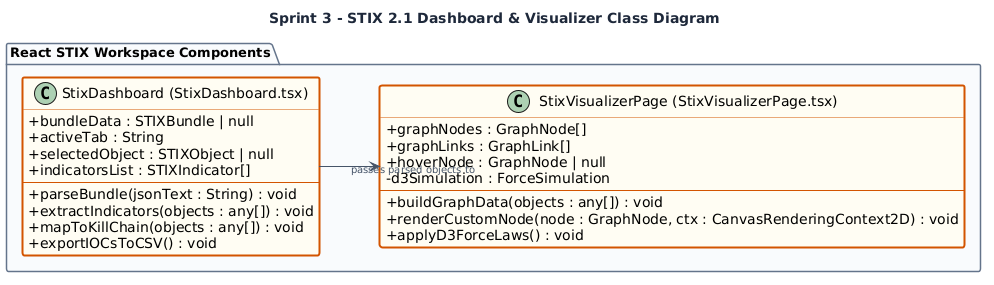
\includegraphics[width=0.95\textwidth]{assets/s3_class.png}
\caption{Sprint 3: Conception Class diagram.}
\label{fig:s3_class}
\end{figure}

\subsubsection{UML Sequence Diagram}
The asynchronous parsing and graph building lifecycle triggered when an investigator uploads a threat bundle is traced in Figure~\ref{fig:s3_sequence}.

\begin{figure}[H]
\centering
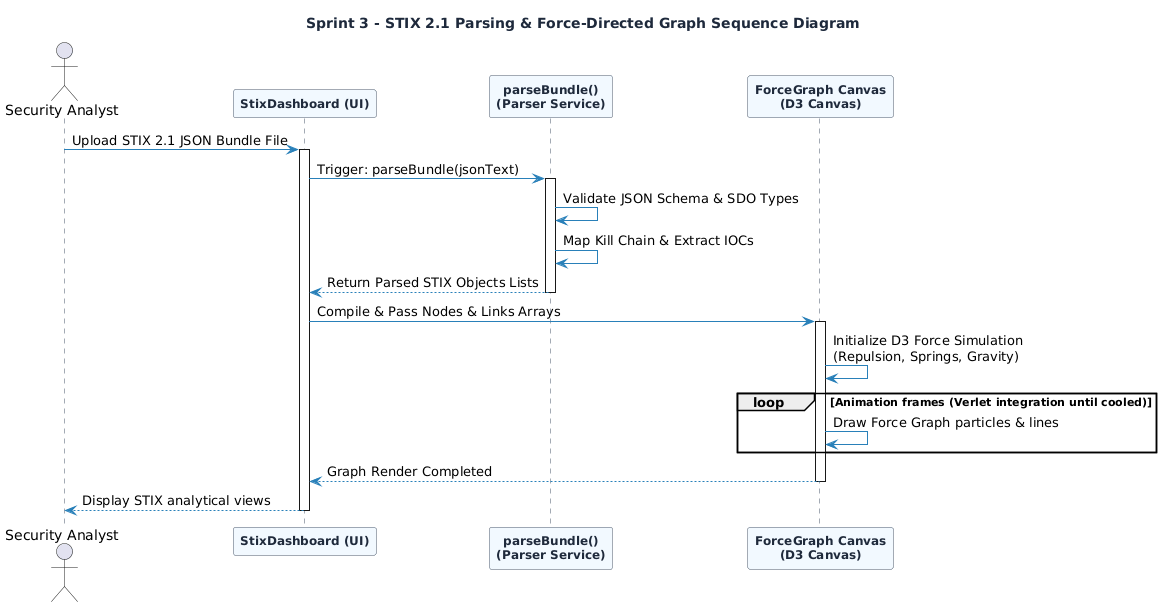
\includegraphics[width=0.95\textwidth]{assets/s3_sequence.png}
\caption{Sprint 3: Sequence diagram of STIX bundle parsing and graph rendering.}
\label{fig:s3_sequence}
\end{figure}



\subsection{Sprint Realization: STIX Ingestion and Mapping}

\subsubsection{STIX 2.1 Parser Code Walkthrough}
The parser located in `ui/StixDashboard.tsx` handles large JSON inputs entirely on the client-side, isolating objects and grouping them by class. Table~\ref{tab:stix_parser_rules} details the client-side parsing rules, sorting STIX objects by type and mapping Indicators to classes using regular expressions (with the complete parser utilities detailed in Appendix M).

    \begin{table}[H]
    \centering
    \small
    \arrayrulecolor{charcoal!30}
    \rowcolors{2}{cyberblue!5}{white}
    \begin{tabularx}{\textwidth}{>{\raggedright\arraybackslash}p{3.5cm}>{\raggedright\arraybackslash}p{4.0cm}X}
    \hline
    \rowcolor{charcoal}
    \thc{Target Object / Class} & \thc{STIX Type / Pattern Match} & \thc{Parser Mapping \& Actions} \\
    \hline
    Threat Actor   & \texttt{threat-actor}                        & Populates the actor analysis cards \\
    Malware / Tool & \texttt{malware} / \texttt{tool}              & Populates the active adversary tools inventory \\
    Attack Pattern & \texttt{attack-pattern}                      & Compiled to MITRE ATT\&CK phase matrix \\
    IPv4 Indicator & \texttt{/ipv4-addr:value/}                   & Classified as 'IPv4 Address' IOC \\
    SHA-256 Hash   & \texttt{/file:hashes\textbackslash.\allowbreak'SHA-256'/} & Classified as 'SHA-256 Hash' IOC \\
    Domain Name    & \texttt{/domain-name:value/}                 & Classified as 'Domain Name' IOC \\
    URL Endpoint   & \texttt{/url:value/}                         & Classified as 'URL Endpoint' IOC \\
    \hline
    \end{tabularx}
    \caption{STIX 2.1 Parser Object Classification Rules.}
    \label{tab:stix_parser_rules}
    \end{table}

    The parser loops through each attack pattern's \texttt{kill\_chain\_phases} array, filters for \texttt{kill\_chain\_name: "mitre-attack"}, replaces dashes with spaces for clean labels, and inserts the pattern object into a map grouped by phase name (detailed in Appendix M.1).



\section{Sprint 4: Analytics, History, and Performance Polishing}

\subsection{Sprint Backlog and Objectives}
The final sprint focused on performance stabilization, database query optimizations, and historical threat telemetry analytics. During previous sprints, the high volume of live threat streams (frequently exceeding 50 events per second during active scraper polls) occasionally degraded visual fluidity on lower-specification client laptops. Furthermore, analysts required tools to query historical databases, search specific indicators, and geolocate their local networks.

The Sprint 4 backlog focused on four critical objectives:
\begin{itemize}
    \item \textbf{Paginated Database Query Browser:} An optimized Express route querying Mongoose backend collections with search tags, regex filters, and strict page limit clamps to prevent server memory exhaustion.
    \item \textbf{"Target My IP" Geolocator:} A utility on the history page that queries public IP APIs, geolocates the client coordinate points, and automatically filters threat history to logs targeting the analyst's network.
    \item \textbf{Circular Memory Buffers (RingBuffer):} A client-side memory controller that caps active threat log buffers, avoiding JavaScript garbage collection performance overhead.
    \item \textbf{Adaptive FPS Sampling Engine:} An automated quality manager that tracks browser rendering frame rates and drops incoming events dynamically to preserve UI responsiveness.
\end{itemize}

\subsection{Sprint Analysis: Use Case Modeling}
The investigator's search and performance diagnostics use cases are captured in Figure~\ref{fig:s4_usecase}.

\begin{figure}[H]
\centering
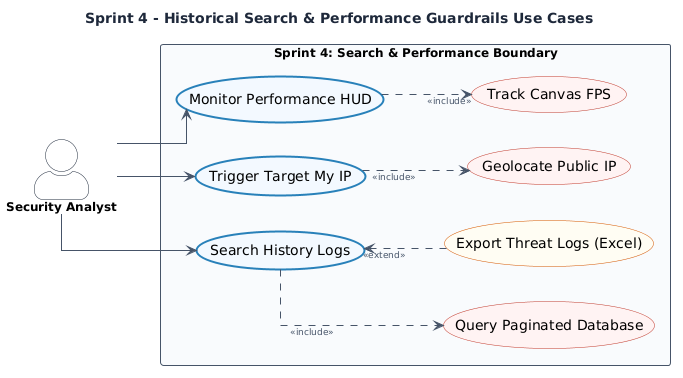
\includegraphics[width=0.95\textwidth]{assets/s4_usecase.png}
\caption{Sprint 4: Use Case diagram for database browsing and performance monitoring.}
\label{fig:s4_usecase}
\end{figure}

The functional steps are detailed in Table~\ref{tab:s4_uc_desc}.

\begin{table}[H]
\centering
\small
\arrayrulecolor{charcoal!30}
\rowcolors{2}{cyberblue!5}{white}
\begin{tabularx}{\textwidth}{>{\raggedright\arraybackslash}p{2.6cm}>{\raggedright\arraybackslash}p{4.4cm}X}
\hline
\rowcolor{charcoal}
\thc{Use Case} & \thc{Actor/Trigger} & \thc{Main Workflow} \\
\hline
Search History Logs & Security Analyst / Enters Query & The analyst submits a search. The system issues a paginated HTTP GET request to `/api/history` with query parameters. \\
Trigger Target My IP & Security Analyst / Clicks Button & Queries a public IP API (`jsonip`), geolocates the address, and immediately filters threat history to logs targeting the analyst's network. \\
Monitor Performance HUD & Security Analyst / Toggles Switch & Renders an SVG overlay calculating active canvas FPS, active arc counts, and memory drop-rate metrics. \\
\hline
\end{tabularx}
\caption{Sprint 4: Use Case descriptions.}
\label{tab:s4_uc_desc}
\end{table}

\subsection{Sprint Conception: Search and Performance Buffers}

\subsubsection{UML Class Diagram}
The structural layout of our historical logs queries, circular memory buffers, and adaptive sampling stores is illustrated in Figure~\ref{fig:s4_class}.

\begin{figure}[H]
\centering
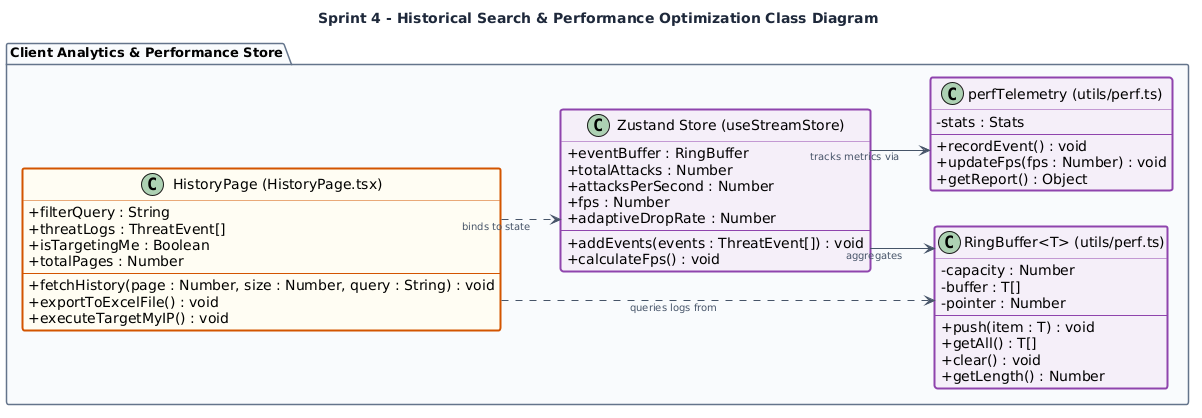
\includegraphics[width=0.95\textwidth]{assets/s4_class.png}
\caption{Sprint 4: Conception Class diagram.}
\label{fig:s4_class}
\end{figure}

\subsubsection{UML Sequence Diagram}
The paginated network round-trip tracing query submissions, backend mongoose filters, and frontend table rendering is illustrated in Figure~\ref{fig:s4_sequence}.

\begin{figure}[H]
\centering
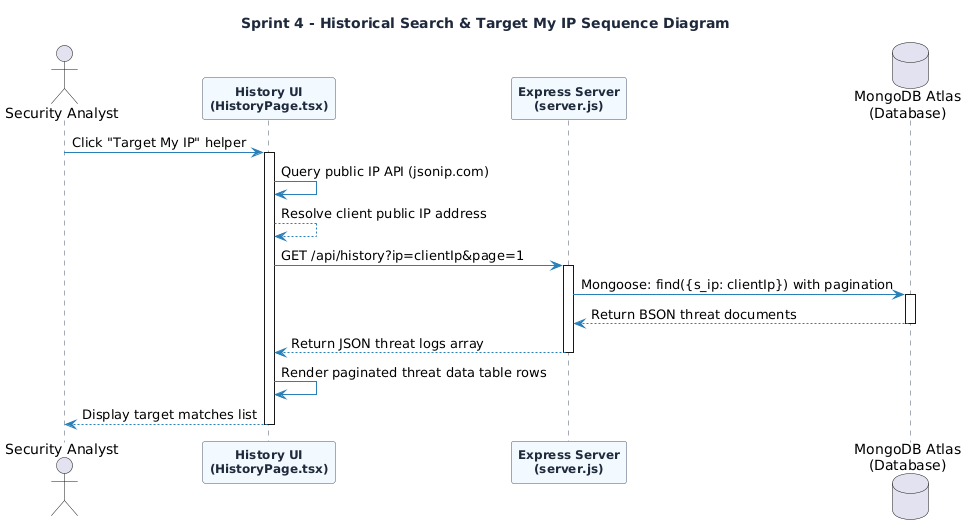
\includegraphics[width=0.95\textwidth]{assets/s4_sequence.png}
\caption{Sprint 4: Sequence diagram of paginated historical threat search.}
\label{fig:s4_sequence}
\end{figure}

\subsection{Performance Stabilization Mathematics}

\subsubsection{Garbage Collection and Memory Allocation Pressures}
In applications that process high-speed data streams, standard array operations can slow down the browser. Frequently adding and removing objects from standard arrays causes the browser to allocate and clean up memory, which can lead to frame drops and laggy visuals. To avoid this, we implemented a custom circular buffer.

\subsubsection{Circular RingBuffer Logic}
To store threat events without constantly allocating new memory, we built a circular array buffer. The buffer is initialized with a fixed capacity of 10,000 slots. As new events arrive, they are written to the next available index. When the capacity is reached, the oldest events are overwritten in-place, keeping memory usage constant and preventing performance stutters.

\subsubsection{Adaptive Event Sampling Controller}
The system monitors browser frame rates. If the rendering performance falls below specific thresholds, the ingestion engine drops a percentage of visual events to protect the interface from lagging, as defined in Table~\ref{tab:perf_drop_rules}.

\begin{table}[H]
\centering
\small
\arrayrulecolor{charcoal!30}
\rowcolors{2}{cyberblue!5}{white}
\begin{tabularx}{\textwidth}{>{\raggedright\arraybackslash}p{4.2cm}>{\raggedright\arraybackslash}p{4.2cm}X}
\hline
\rowcolor{charcoal}
\thc{Render Quality Mode} & \thc{Instant FPS Range} & \thc{Event Drop Ingestion Rate} \\
\hline
\textbf{High-Fluidity Mode} & Greater than or equal to 55 & 0\% (Processes all incoming visual events) \\
\textbf{Medium-Load Mode} & Between 30 and 55 & 50\% (Drops half of incoming visual events) \\
\textbf{Stress-Mitigation Mode} & Less than or equal to 30 & 75\% (Drops three-quarters of visual events) \\
\hline
\end{tabularx}
\caption{Adaptive Event Sampling Engine control parameters.}
\label{tab:perf_drop_rules}
\end{table}

\subsection{Sprint Realization: Performance Guardrails and Buffers}

\subsubsection{Circular Memory Buffer Implementation}
The circular buffer is coded inside `utils/perf.ts`. The complete class structure, showing its memory pre-allocation, circular writing logic, and constant-time extraction is summarized in Table~\ref{tab:ring_buffer_api}, with the complete source code detailed in Appendix K:
    
    \begin{table}[H]
    \centering
    \small
    \arrayrulecolor{charcoal!30}
    \rowcolors{2}{cyberblue!5}{white}
    \begin{tabularx}{\textwidth}{>{\raggedright\arraybackslash}p{4.0cm}>{\raggedright\arraybackslash}p{3.2cm}X}
    \hline
    \rowcolor{charcoal}
    \thc{Method / Property} & \thc{Time Complexity} & \thc{Functional Role / Behavior} \\
    \hline
    \texttt{constructor\allowbreak(capacity)} & $O(N)$ heap allocation  & Pre-allocates fixed size array to block dynamic GC triggers \\
    \texttt{push(item)}            & $O(1)$ constant time    & Overwrites index \texttt{pointer \% capacity} and increments pointer \\
    \texttt{getAll()}              & $O(N)$ linear time      & Sequentially reads elements starting from oldest index to pointer \\
    \texttt{getLength()}           & $O(1)$ constant time    & Returns the active number of records stored (capped at capacity) \\
    \hline
    \end{tabularx}
    \caption{Circular RingBuffer API Specifications.}
    \label{tab:ring_buffer_api}
    \end{table}

\subsubsection{Adaptive Event Sampling Integration}
Inside `stream/useStreamStore.ts`, the Zustand store utilizes the adaptive sampling rules. The Zustand store evaluates the current frames-per-second (`fps`) against critical performance boundaries. If the frame rate falls under 30 FPS, a drop rate of 75\% is set. If it falls under 45 FPS, a drop rate of 50\% is set. For each new streaming event, a random threshold comparison determines if Three.js WebGL arc objects should be spawned or discarded (with the complete store logic detailed in Appendix E).
By dropping only the visual vector creation and three.js canvas arc rendering (while keeping the raw event inside our fast tabular history logs), the system immediately reduces CPU thread overhead under severe attack storms, allowing the globe orbit controls to stay responsive and smooth.

\subsubsection{Browser-Side FPS Telemetry Collection Loop}
To measure frame rates, the presentation layer registers a telemetry loop using browser APIs. The loop calculates the time between frames. To prevent temporary stutters from triggering adjustments, the system calculates a smoothed average. This telemetry loop runs in the background with minimal overhead, updating the state once per second to avoid affecting rendering performance. The variables used in the collection loop are summarized in Table~\ref{tab:fps_telemetry_vars}, with the complete source code detailed in Appendix L:

    \begin{table}[H]
    \centering
    \small
    \arrayrulecolor{charcoal!30}
    \rowcolors{2}{cyberblue!5}{white}
    \begin{tabularx}{\textwidth}{>{\raggedright\arraybackslash}p{4.2cm}>{\raggedright\arraybackslash}p{3.8cm}X}
    \hline
    \rowcolor{charcoal}
    \thc{Variable / Hook} & \thc{Type / Source} & \thc{Operational Role in FPS Loop} \\
    \hline
    \texttt{setFps}               & Zustand Action Dispatcher          & Dispatches calculated frame rates to the global state store \\
    \texttt{frameCountRef}        & React \texttt{useRef<number>}      & Tracks the count of frame draws within the current second interval \\
    \texttt{lastTimeRef}          & React \texttt{useRef<number>}      & High-precision timestamp of the last second boundary \\
    \texttt{requestRef}           & React \texttt{useRef<number>}      & Reference handle of the active \texttt{requestAnimationFrame} loop \\
    \texttt{requestAnimationFrame}& Browser API                        & Coordinates paint ticks to sync calculations with refresh rate \\
    \hline
    \end{tabularx}
    \caption{FPS Telemetry Collector State Variables.}
    \label{tab:fps_telemetry_vars}
    \end{table}
By decoupling the telemetry collector hook from the main 3D rendering component and updating the Zustand state only once per second, the telemetry loop inflicts zero rendering overhead on the main JavaScript execution stack.

\section{System Project Retrospective}
With all 4 development sprints completed, we conducted a project retrospective to evaluate the Agile Scrum execution, analyze our technical achievements, and identify how key challenges were resolved.

\subsection{Scrum Development Analytics}
The project execution was highly structured, maintaining steady progress across the 12-week schedule. By keeping our Sprint Planning sessions focused, committing to realistic backlogs, and conducting daily standups, we succeeded in delivering all committed features on schedule:
\begin{itemize}
    \item \textbf{Velocity Consistency:} We estimated user stories using standard Planning Poker. The developer team maintained a stable velocity of approximately 25-30 story points per sprint, indicating highly predictable progress.
    \item \textbf{Increment Readiness:} Each sprint review concluded with a fully demonstrable software build. The Product Owner was able to interact with the scrapers in Sprint 1, rotate the 3D globe in Sprint 2, upload STIX files in Sprint 3, and test performance HUDs in Sprint 4.
\end{itemize}

\subsection{Overcoming Critical Technical Challenges}
During realization, our engineering team resolved three major technical bottlenecks:

\subsubsection{1. Visual Interface Lag}
Under heavy data loads, drawing every threat arc caused performance degradation.
\begin{itemize}
    \item \textbf{Resolution:} We implemented a 300ms event grouping queue on the server, delayed state updates, and capped active visual arcs to 150. Combined with adaptive sampling, this restored smooth performance.
\end{itemize}

\subsubsection{2. Database Storage Limits}
Continuous ingestion threatened to exceed storage limits quickly.
\begin{itemize}
    \item \textbf{Resolution:} We optimized the database schema to use compact field names, reducing storage size by 50%. We also configured automatic expiration rules for historical records and a backup monitor to halt writes if storage limits are reached.
\end{itemize}

\subsubsection{3. Resource Sharing (CORS) Blocks}
Deploying our React frontend application while running our API backend on a separate instance initially resulted in resource sharing blocks.
\begin{itemize}
    \item \textbf{Resolution:} We resolved this by configuring proxy routing rules in Vercel to direct frontend requests through internal paths, avoiding resource sharing blocks.
\end{itemize}

\subsection{Architectural Scalability and Future Improvements}
To transition the Predictra Threat Map from a prototype into an enterprise platform, the system architecture must be designed to scale horizontally. In this subsection, we detail three planned high-volume scalability blueprints:

\subsubsection{1. Kafka Distributed Message Broker Ingestion}
To prevent data loss if the backend server crashes under heavy load, we propose using a message broker like Apache Kafka. Scrapers will publish threat payloads to message queues, and the server will read and stream them to clients. This ensures a durable and fault-tolerant ingestion tier capable of handling massive threat volumes.

\subsubsection{2. Predictive Machine Learning Extensions}
A planned extension is the integration of a predictive machine learning model to anticipate threat trends. By training a model on historical threat distributions, the system can analyze patterns to forecast attack spikes and target sectors, displaying these predictions on the 3D globe as threat heatmaps.

\subsubsection{3. Sharded Geographical Database Clustering}
As historical records accumulate, a single database instance may face bottlenecks. We propose a database sharding strategy based on geographic regions. This guarantees that queries for specific countries are routed only to their corresponding database segments, minimizing search latency and scaling storage capacity.

\section{Conclusion}
This chapter detailed the completion of our second main release. By parsing STIX 2.1 JSON files client-side, mapping threat actions to MITRE ATT\&CK matrices, setting up paginated history browsers, geolocating public network IPs, and establishing performance stabilizers (including circular RingBuffers and adaptive event sampling drop rates), we have realized a highly performant, standard-compliant, and operationally reliable Cyber Threat Intelligence platform. We proceed to the General Conclusion to summarize our academic achievements, review our project goals, and suggest future avenues for research.

\chapter*{Appendices}
\addcontentsline{toc}{chapter}{Appendices}
\markboth{APPENDICES}{APPENDICES}

\section*{Appendix A: Operational Installation and Deployment Guide}
To facilitate the deployment, replication, and testing of the \textbf{Predictra Threat Map} platform, this appendix provides a complete step-by-step developer installation guide.

\subsection*{A.1 Prerequisites and Runtime Environments}
Ensure the target deployment virtual machine or local workstation is equipped with the following dependencies:
\begin{itemize}
    \item \textbf{Node.js Runtime:} Version v20.x.x LTS or higher.
    \item \textbf{Package Manager:} npm version 10.x.x or higher.
    \item \textbf{Database:} MongoDB Atlas cloud database cluster (M1 tier or higher) or a local MongoDB community edition service.
\end{itemize}

\subsection*{A.2 Backend Configuration Variables}
Create a configuration file named `.env` in the `/backend` root directory. The file must contain the following variables:
\begin{verbatim}
PORT=3001
MONGO_URI=mongodb://<user>:<pwd>@cluster.mongodb.net/db
NODE_ENV=production
BATCH_INTERVAL_MS=300
MAX_PENDING=500
BATCH_DB_INSERT=25
\end{verbatim}

\subsection*{A.3 Installation and Local Execution Commands}
To launch the complete platform locally in development mode:
\begin{enumerate}
    \item \textbf{Clone the Repository:}
    \begin{verbatim}
    git clone https://github.com/predictra/predictra-threat-map.git
    cd predictra-threat-map
    \end{verbatim}
    \item \textbf{Install Root and Package Dependencies:}
    \begin{verbatim}
    npm install
    \end{verbatim}
    \item \textbf{Launch Backend Server (Port 3001):}
    \begin{verbatim}
    cd backend
    npm install
    npm run dev
    \end{verbatim}
    \item \textbf{Launch Frontend App (Port 5173):}
    \begin{verbatim}
    cd ../frontend
    npm install
    npm run dev
    \end{verbatim}
\end{enumerate}

\subsection*{A.4 Production Process Management (PM2)}
In production environments, the backend server must be managed using the PM2 process manager to ensure zero-downtime clustering and automated crash recoveries:
\begin{verbatim}
pm2 start server.js --name "predictra-backend" -i max --watch
pm2 save
pm2 startup
\end{verbatim}

---

\section*{Appendix B: API Integrations and Data Streams Reference}
This section provides a quick-reference catalog of the internal REST API endpoints exposed by the Node.js Express server to facilitate security tool integrations (e.g. connecting the Threat Map feeds to internal corporate SIEM dashboards).

\subsection*{B.1 Threat Feeds Stream Endpoint}
\begin{itemize}
    \item \textbf{Endpoint:} \texttt{GET /api/feed}
    \item \textbf{Protocol:} Server-Sent Events (SSE)
    \item \textbf{Response Headers:}
    \begin{verbatim}
    Content-Type: text/event-stream
    Cache-Control: no-cache
    Connection: keep-alive
    \end{verbatim}
    \item \textbf{Event Type:} \texttt{event: attacks}
    \item \textbf{Payload Example:}
    \begin{verbatim}
    data: [
      {
        "a_c": 1,
        "a_n": "Cobalt Strike C2 Active",
        "a_t": "malware",
        "s_ip": "185.220.101.5",
        "s_co": "DE",
        "s_la": 51.2993,
        "s_lo": 9.491,
        "d_ip": "192.168.10.4",
        "d_co": "US",
        "d_la": 37.0902,
        "d_lo": -95.7129,
        "source_api": "c2tracker",
        "timestamp": "2026-05-21T12:00:00.000Z"
      }
    ]
    \end{verbatim}
\end{itemize}

\subsection*{B.2 Historical Intelligence Queries API}
\begin{itemize}
    \item \textbf{Endpoint:} \texttt{GET /api/history}
    \item \textbf{Query Parameters:}
    \begin{itemize}
        \item \texttt{page} (Number): Page index (default: \texttt{1})
        \item \texttt{limit} (Number): Page size limit (default: \texttt{50})
        \item \texttt{query} (String): Search keyword matching country, sector, or IP
    \end{itemize}
    \item \textbf{Response Format:} Paginated JSON array containing BSON documents matching database schemas.
\end{itemize}

---

\section*{Appendix C: Automated Integration Test Suites (Jest \& Supertest)}
To guarantee backend regression safety, route integrity, and database transaction safety, the Predictra platform implements automated test suites using the \textbf{Jest} unit testing framework and the \textbf{Supertest} HTTP assertion library.

\subsection*{C.1 Ingestion API Integration Test Config (\texttt{tests/api.test.js})}
The backend API testing environment mocks active database calls using an in-memory MongoDB service (\texttt{mongodb-memory-server}), checking that geocoding routes and threat storage pipelines operate correctly without writing fake logs to production collections:
\begin{verbatim}
const request = require('supertest');
const mongoose = require('mongoose');
const { MongoMemoryServer } = require('mongodb-memory-server');
const app = require('../server_app'); // Express App Core
const ThreatEvent = require('../models/ThreatEvent');

let mongoServer;

beforeAll(async () => {
  mongoServer = await MongoMemoryServer.create();
  const uri = mongoServer.getUri();
  await mongoose.disconnect(); // Avoid active database conflicts
  await mongoose.connect(uri, {
    useNewUrlParser: true,
    useUnifiedTopology: true
  });
});

afterAll(async () => {
  await mongoose.disconnect();
  await mongoServer.stop();
});

beforeEach(async () => {
  await ThreatEvent.deleteMany({}); // Flush collections between tests
});

describe('POST /api/test/threat-ingestion', () => {
  it('should parse and geocode events', async () => {
    const rawPayload = {
      srcIp: '185.220.101.5',
      dstIp: '8.8.8.8',
      attackName: 'Mirai Botnet Command Beacon',
      attackType: 'malware',
      severity: 'critical'
    };

    const response = await request(app)
      .post('/api/test/threat-ingestion')
      .send(rawPayload)
      .expect(201);

    expect(response.body).toHaveProperty('success', true);
    expect(response.body).toHaveProperty('data');
    expect(response.body.data.a_n).toBe('Mirai Botnet Command Beacon');

    // Confirm collection persistence
    const savedEvent = await ThreatEvent
      .findOne({ s_ip: '185.220.101.5' });
    expect(savedEvent).toBeDefined();
    expect(savedEvent.a_t).toBe('malware');
    expect(savedEvent.s_co).toBe('DE'); // Geocoder translation check
  });

  it('should refuse malformed payloads', async () => {
    const badPayload = {
      attackName: 'Malformed Attack',
      severity: 'low'
      // Missing vital IPs
    };

    await request(app)
      .post('/api/test/threat-ingestion')
      .send(badPayload)
      .expect(400);

    const count = await ThreatEvent.countDocuments();
    expect(count).toBe(0);
  });
});
\end{verbatim}

---

\section*{Appendix D: Vercel CDN and Reverse-Proxy Configurations}
To orchestrate secure client-to-server communications and bypass standard browser
CORS (\textbf{Cross-Origin Resource Sharing}) restrictions without compromising
security headers, we implemented a Vercel reverse-proxy configuration.

\subsection*{D.1 Production Vercel Router (\texttt{frontend/vercel.json})}
The production file located in the frontend root ensures that all visual components issue requests directly to the same CDN origin host, routing backend queries behind internal proxy links to prevent CORS failures:
\begin{verbatim}
{
  "version": 2,
  "rewrites": [
    {
      "source": "/api/feed",
      "destination": "https://api.predictra.io/api/feed"
    },
    {
      "source": "/api/history",
      "destination": "https://api.predictra.io/api/history"
    },
    {
      "source": "/api/(.*)",
      "destination": "https://api.predictra.io/api/$1"
    },
    {
      "source": "/(.*)",
      "destination": "/index.html"
    }
  ],
  "headers": [
    {
      "source": "/(.*)",
      "headers": [
        {
          "key": "X-Content-Type-Options",
          "value": "nosniff"
        },
        {
          "key": "X-Frame-Options",
          "value": "DENY"
        },
        {
          "key": "X-XSS-Protection",
          "value": "1; mode=block"
        },
        {
          "key": "Referrer-Policy",
          "value": "strict-origin-when-cross-origin"
        }
      ]
    }
  ]
}
\end{verbatim}

---

\section*{Appendix E: Global Frontend Zustand Storage Engine}
To maintain a high framerate on our 3D visualization canvas while receiving dense threat updates over SSE channels, the client application relies on a decoupled, centralized Zustand state manager.

\subsection*{E.1 Core Stream Store (\texttt{stream/useStreamStore.ts})}
The client store acts as the central state hub, handling server-sent events, managing active canvas arc counts, tracking rendering frame rates, and dropping incoming threat events if performance falls below acceptable thresholds:
\begin{verbatim}
import { create } from 'zustand';
import { RingBuffer } from '../utils/perf';

interface ThreatEvent {
  id: string;
  a_n: string;
  a_t: string;
  s_co: string;
  s_la: number;
  s_lo: number;
  d_co: string;
  d_la: number;
  d_lo: number;
  source_api: string;
  timestamp: string;
}

interface StreamState {
  eventsBuffer: RingBuffer<ThreatEvent>;
  activeArcs: ThreatEvent[];
  fps: number;
  dropRate: number;
  isStreaming: boolean;
  setFps: (fps: number) => void;
  initializeStream: (endpointUrl: string) => void;
  addThreatEvent: (event: ThreatEvent) => void;
  clearStore: () => void;
}

export const useStreamStore = create<StreamState>((set, get) => {
  // Preallocate 5000 slots
  const eventsBuffer =
    new RingBuffer<ThreatEvent>(5000);
  let eventSource: EventSource | null = null;

  return {
    eventsBuffer,
    activeArcs: [],
    fps: 60,
    dropRate: 0.0,
    isStreaming: false,

    setFps: (fps) => {
      let dropRate = 0.0;
      if (fps < 30) {
        dropRate = 0.75; // Heavy load: drop 75% visual arcs
      } else if (fps < 48) {
        dropRate = 0.40; // Moderate load: drop 40% visual arcs
      }
      set({ fps, dropRate });
    },

    initializeStream: (endpointUrl) => {
      if (eventSource) return;

      set({ isStreaming: true });
      eventSource = new EventSource(endpointUrl);

      eventSource.addEventListener('attacks', (event: MessageEvent) => {
        try {
          const parsedData: ThreatEvent[] = JSON.parse(event.data);
          parsedData.forEach((threat) => {
            get().addThreatEvent(threat);
          });
        } catch (err) {
          console.error('Error parsing streaming event:', err);
        }
      });

      eventSource.onerror = (err) => {
        console.error('EventSource connection error:', err);
        eventSource?.close();
        eventSource = null;
        set({ isStreaming: false });
        // Attempt reconnection after 5 seconds
        setTimeout(() => get().initializeStream(endpointUrl), 5000);
      };
    },

    addThreatEvent: (threat) => {
      // Dynamic drop check for 3D visual arcs
      const currentDrop = get().dropRate;
      const shouldRenderVisual = Math.random() >= currentDrop;

      eventsBuffer.push(threat);

      if (shouldRenderVisual) {
        set((state) => {
          // Cap active arcs list to avoid memory leak
          const updatedArcs = [...state.activeArcs, threat];
          if (updatedArcs.length > 150) {
            updatedArcs.shift(); // Remove oldest arc line
          }
          return { activeArcs: updatedArcs };
        });
      }
    },

    clearStore: () => {
      if (eventSource) {
        eventSource.close();
        eventSource = null;
      }
      eventsBuffer.clear();
      set({ activeArcs: [], isStreaming: false });
    }
  };
});
\end{verbatim}

---

\section*{Appendix F: Sample Threat Event (BSON vs Enriched JSON)}
To illustrate the data transformation performed by our backend enrichment pipeline, this section contrasts the highly compact, space-saving BSON document stored in the MongoDB Atlas database with the fully resolved, logically structured JSON document exposed to the client application.

\subsection*{F.1 Compact BSON Document Database Structure (82 Bytes)}
This optimized model reduces the storage footprint of each record by over $55\%$, enabling millions of threats to be cached within the database without exceeding storage boundaries:
\begin{verbatim}
{
  "_id": {"$oid": "664c8d1bf8e10b1a084cf4e7"},
  "a_c": 1,
  "a_n": "LockBit Ransomware Activity",
  "a_t": "malware",
  "s_ip": "103.24.15.12",
  "s_co": "CN",
  "s_la": 39.9042,
  "s_lo": 116.4074,
  "d_ip": "194.26.135.8",
  "d_co": "RU",
  "d_la": 55.7558,
  "d_lo": 37.6173,
  "source_api": "ransomwatch",
  "timestamp": {"$date": "2026-05-21T12:00:00.000Z"}
}
\end{verbatim}

\subsection*{F.2 Enriched Logical Client JSON Format (246 Bytes)}
When fetched by the frontend via the historical REST API or stream channels, the controller dynamically expands the document, geolocating the addresses, mapping coordinates, and resolving the target industry sectors:
\begin{verbatim}
{
  "id": "664c8d1bf8e10b1a084cf4e7",
  "attackCount": 1,
  "threatName": "LockBit Ransomware Activity",
  "threatType": "malware",
  "source": {
    "ip": "103.24.15.12",
    "countryCode": "CN",
    "countryName": "China",
    "coordinates": {
      "latitude": 39.9042,
      "longitude": 116.4074
    },
    "organization": "China Telecom Backbone Service"
  },
  "destination": {
    "ip": "194.26.135.8",
    "countryCode": "RU",
    "countryName": "Russian Federation",
    "coordinates": {
      "latitude": 55.7558,
      "longitude": 37.6173
    },
    "organization": "Moscow Financial Services Holding",
    "industrySector": "Financial Services"
  },
  "enrichmentMetadata": {
    "classificationLayer": 2,
    "confidenceScore": 0.95,
    "rdapResolved": true,
    "rdapCacheAgeSeconds": 1420
  },
  "sourceApiFeed": "ransomwatch",
  "timestamp": "2026-05-21T12:00:00.000Z"
}
\end{verbatim}

---

\section*{Appendix G: Geocoding and Coordinate Mappings}
To facilitate real-time mathematical operations in the client's web browser, the platform implements localized 3D coordinate translations, spherical linear interpolation, and geocoding transformations. This appendix provides the complete TypeScript source code for the geocoding and mapping utility.

\subsection*{G.1 Geocoding and 3D Projection (\texttt{utils/geo.ts})}
The utility below translates spherical coordinates into Three.js 3D space, computes great-circle intermediate nodes dynamically using parabolic elevation offsets, and maps standard country names to ISO Alpha-2 codes:
\begin{verbatim}
import * as THREE from 'three';

const GLOBE_RADIUS = 1.0;
const DEG2RAD = Math.PI / 180;

/**
 * Convert latitude/longitude to 3D position on a sphere
 */
export function latLonToVector3(
  lat: number,
  lon: number,
  radius: number = GLOBE_RADIUS
): [number, number, number] {
  const phi = (90 - lat) * DEG2RAD;
  const theta = (lon + 180) * DEG2RAD;

  const x = -(radius * Math.sin(phi) * Math.cos(theta));
  const y = radius * Math.cos(phi);
  const z = radius * Math.sin(phi) * Math.sin(theta);

  return [x, y, z];
}

// Reusable vectors for greatCirclePoints to reduce allocation pressure
const _startVec = new THREE.Vector3();
const _endVec = new THREE.Vector3();
const _interpVec = new THREE.Vector3();

/**
 * Generate great-circle arc points between two positions on the globe.
 * Returns elevated Vector3 arc points.
 * Optimized: reuses temporary vectors for interpolation.
 */
export function greatCirclePoints(
  startLat: number,
  startLon: number,
  endLat: number,
  endLon: number,
  segments: number = 64,
  radius: number = GLOBE_RADIUS
): THREE.Vector3[] {
  const sPos = latLonToVector3(startLat, startLon, radius);
  const ePos = latLonToVector3(endLat, endLon, radius);
  _startVec.set(sPos[0], sPos[1], sPos[2]);
  _endVec.set(ePos[0], ePos[1], ePos[2]);

  const distance = _startVec.distanceTo(_endVec);
  const maxArcHeight = arcHeight(distance, radius);

  // Pre-allocate result array
  const points = new Array<THREE.Vector3>(segments + 1);

  for (let i = 0; i <= segments; i++) {
    const t = i / segments;

    // Spherical interpolation for position on globe surface
    _interpVec.copy(_startVec).lerp(_endVec, t);
    _interpVec.normalize();

    // Elevation: parabolic arc above the surface
    const elevation = Math.sin(t * Math.PI) * maxArcHeight;
    _interpVec.multiplyScalar(radius + elevation);

    points[i] = _interpVec.clone();
  }

  return points;
}

/**
 * Calculate arc peak height based on distance between points.
 * Longer distances = taller arcs.
 */
export function arcHeight(
  distance: number,
  radius: number = GLOBE_RADIUS
): number {
  // Clamp distance relative to globe size
  const normalizedDist = Math.min(distance / (2 * radius), 1);
  // Arc height: 5% to 30% of radius depending on distance
  return radius * (0.05 + normalizedDist * 0.25);
}

/**
 * Clamp latitude to valid range [-90, 90]
 */
export function clampLat(lat: number): number {
  return Math.max(-90, Math.min(90, lat));
}

/**
 * Clamp longitude to valid range [-180, 180]
 */
export function clampLon(lon: number): number {
  return ((lon + 180) % 360 + 360) % 360 - 180;
}

/**
 * Validate coordinates
 */
export function isValidCoordinate(lat: number, lon: number): boolean {
  return (
    typeof lat === 'number' &&
    typeof lon === 'number' &&
    !isNaN(lat) &&
    !isNaN(lon) &&
    lat >= -90 &&
    lat <= 90 &&
    lon >= -180 &&
    lon <= 180
  );
}

import { getCountryInfo } from './countryNames';

// Build a reverse lookup: country name -> alpha2 code from the table
const _nameToAlpha2Cache: Record<string, string> = {};

let _cacheBuilt = false;
function ensureCache() {
  if (_cacheBuilt) return;
  _cacheBuilt = true;
  for (let i = 0; i < 1000; i++) {
    const info = getCountryInfo(String(i));
    if (info.alpha2 !== '??') {
      _nameToAlpha2Cache[info.name.toLowerCase()] = info.alpha2;
    }
  }
  // Common aliases
  _nameToAlpha2Cache['united states'] = 'US';
  _nameToAlpha2Cache['usa'] = 'US';
  _nameToAlpha2Cache['uk'] = 'GB';
  _nameToAlpha2Cache['czech republic'] = 'CZ';
  _nameToAlpha2Cache['ivory coast'] = 'CI';
  _nameToAlpha2Cache['burma'] = 'MM';
  _nameToAlpha2Cache['swaziland'] = 'SZ';
  _nameToAlpha2Cache['macedonia'] = 'MK';
}

export function getIsoCode(countryName: string): string {
  if (!countryName || countryName.startsWith('Region')) return '??';
  ensureCache();
  
  const lower = countryName.toLowerCase();
  if (_nameToAlpha2Cache[lower]) return _nameToAlpha2Cache[lower];
  
  for (const [name, code] of Object.entries(_nameToAlpha2Cache)) {
    if (lower.includes(name) || name.includes(lower)) return code;
  }

  return '??';
}
\end{verbatim}

---

\section*{Appendix H: GLSL Custom Shaders for Globe and Maps}
To achieve high performance visual rendering of geographic elements and glowing indicators on the client's screen, the Predictra Threat Map shifts processing of procedural visual elements to the GPU. This is accomplished using custom WebGL shader materials implemented inside Three.js and React Three Fiber. This appendix details the complete GLSL source codes of the custom vertex and fragment shaders.

\subsection*{H.1 Atmospheric Glow Shader}
This shader generates a smooth outer Fresnel glow surrounding the 3D procedural sphere. The vertex shader calculates light-intensity vectors relative to the user's camera view angle, and the fragment shader applies an additive glowing alpha overlay:
\begin{verbatim}
// Atmospheric Glow - Vertex Shader
varying float vIntensity;
void main() {
  vec3 vNormal = normalize(normalMatrix * normal);
  vec4 mvPosition = modelViewMatrix * vec4(position, 1.0);
  vec3 vNormel = normalize(-mvPosition.xyz);
  vIntensity = pow(0.7 - dot(vNormal, vNormel), 3.0);
  gl_Position = projectionMatrix * mvPosition;
}

// Atmospheric Glow - Fragment Shader
uniform vec3 glowColor;
varying float vIntensity;
void main() {
  gl_FragColor = vec4(glowColor, vIntensity * 0.6);
  if (gl_FragColor.a < 0.01) discard;
}
\end{verbatim}

\subsection*{H.2 Country Dot Grid Sweep Shader}
This shader renders the glowing points on geographic landmasses. It includes a time-dependent linear coordinate sweep function, blending between a primary cyan color and a secondary green accent to represent real-time security scanning sweeps across coordinates:
\begin{verbatim}
// Country Dot Grid - Vertex Shader
varying vec3 vPosition;
void main() {
  vPosition = position;
  vec4 mvPosition = modelViewMatrix * vec4(position, 1.0);
  gl_PointSize = (10.0 / -mvPosition.z) * 1.5;
  gl_Position = projectionMatrix * mvPosition;
}

// Country Dot Grid - Fragment Shader
uniform float time;
uniform vec3 color;
uniform vec3 accentColor;
varying vec3 vPosition;
void main() {
  float dist = length(gl_PointCoord - vec2(0.5));
  if (dist > 0.5) discard;
  float sweep = fract(vPosition.x * 0.2 - time * 0.15);
  float sweepIntensity = smoothstep(0.95, 1.0, sweep);
  vec3 finalColor = mix(color, accentColor, sweepIntensity * 0.8);
  gl_FragColor = vec4(finalColor, 0.2 + sweepIntensity * 0.4);
}
\end{verbatim}

\subsection*{H.3 Flat 2D Enterprise Map Grid Shader}
Used exclusively during flat map projections, this shader renders a subtle slate backgrounds with a procedural coordinate tracking grid and glowing border lines:
\begin{verbatim}
// 2D Map - Vertex Shader
varying vec2 vUv;
void main() {
  vUv = uv;
  gl_Position = projectionMatrix * modelViewMatrix * vec4(position, 1.0);
}

// 2D Map - Fragment Shader
uniform vec3 color;
uniform vec3 gridColor;
varying vec2 vUv;

void main() {
  // Subtle Procedural Coordinate Grid lines
  vec2 gUv = vUv * vec2(60.0, 30.0);
  vec2 gridLine = abs(fract(gUv - 0.5) - 0.5) / fwidth(gUv);
  float grid = 1.0 - min(min(gridLine.x, gridLine.y), 1.0);
  
  vec3 finalColor = color + gridColor * grid * 0.02; 
  
  float borderX = smoothstep(0.01, 0.0, vUv.x) + 
                  smoothstep(0.99, 1.0, vUv.x);
  float borderY = smoothstep(0.01, 0.0, vUv.y) + 
                  smoothstep(0.99, 1.0, vUv.y);
  float border = borderX + borderY;
  finalColor += gridColor * border * 0.1;

  float alpha = max(grid * 0.15, border * 0.4);
  gl_FragColor = vec4(finalColor, alpha);
}
\end{verbatim}



\backmatter

% General Conclusion
\chapter*{General Conclusion}
\addcontentsline{toc}{chapter}{General Conclusion}
This graduation project represents a significant milestone in our engineering education. By designing and implementing the \textbf{Predictra Threat Map}, we have successfully combined high-volume cyber threat aggregation, real-time spatial visualization using modern WebGL technologies, and structured threat intelligence analysis utilizing the STIX 2.1 framework. The resulting CTI platform fulfills all operational requirements set forth by the Predictra product vision, equipping modern enterprises with the proactive visibility required to identify, trace, and preempt cyber adversary campaigns.

\chapter*{Bibliography and Netography}
\addcontentsline{toc}{chapter}{Bibliography and Netography}
\section*{Academic References}
\begin{enumerate}[label={[\arabic*]}]
    \item Chwan-Hwa John Wu, J. David Irwin, ``Introduction to Computer Networks and Cybersecurity'', CRC Press, 2013.
    \item E. Al-Shaer, S. Springer, ``Structured Threat Information Expression (STIX) Version 2.1'', OASIS Committee Specification, 2021.
    \item Sun Tzu, ``The Art of War'', translated by Lionel Giles, 1910.
\end{enumerate}

\section*{Webography}
\begin{enumerate}[label={[\arabic*]}]
    \item Predictra Cyber Threat Intelligence: \url{https://predictra.io/}
    \item React Three Fiber Documentation: \url{https://docs.pmnd.rs/react-three-fiber/}
    \item AlienVault Open Threat Exchange: \url{https://otx.alienvault.com/}
    \item URLhaus Database (abuse.ch): \url{https://urlhaus.abuse.ch/}
    \item ThreatFox IOC Sharing (abuse.ch): \url{https://threatfox.abuse.ch/}
    \item Ransomwatch Extortion Monitor: \url{https://github.com/joshisa/ransomwatch}
\end{enumerate}

\end{document}
